\documentclass{article}
\usepackage[utf8]{inputenc}
\usepackage{bbold, mathtools, amsthm, setspace}
%\usepackage{figcaps}
%\printfigures
%\doublespacing
\usepackage[colorlinks,hypertexnames=true,citecolor=blue]{hyperref} 
\usepackage{natbib}
\usepackage{tikz}
\usepackage{pgfplots}
\usepackage{appendix}
\bibliographystyle{agsm}
\setcitestyle{authoryear,open={(},close={)}}
\newtheorem{theorem}{Theorem}
\setlength{\parskip}{1 em}
\newcommand{\V}{\mathbb{V}}
\newcommand{\E}{\mathbb{E}}
\newcommand{\R}{\mathbb{R}}

\title{A re-examination of the foundations of the\\ cost of capital for regulatory purposes}
%\title{On the term of the cost of capital and the use of the `on-the-day rate' versus the `trailing average approach'}
\author{Darryl Biggar\footnote{Adjunct Associate Professor, Monash University.}}
\date{March 2023}

\begin{document}

\maketitle

\begin{abstract}
\noindent
%Few issues are as hotly contested in public utility regulatory proceedings as the choice of the cost of capital. In Australia there has been virtually continuous debate in regulatory proceedings over the last two decades over fundamental concepts such as the appropriate term of the cost of capital, and the appropriate method for estimating the cost of debt. 
In regulatory proceedings, few issues are more hotly debated than the cost of capital. This article formalises the theoretical foundation of cost of capital estimation for regulatory purposes. Several common regulatory practices lack a solid foundation in the theory.  For example, the common practice of estimating a single cost of capital for the regulated firm suffers from a circularity problem, especially in the context of a multi-year regulatory period. In addition, the relevant cost of debt cannot be estimated using the yield-to-maturity on a corporate bond. We suggest possible directions for reform of cost of capital practices in regulatory proceedings.
%
%The typical approach is to estimate the cost of capital as a weighted average of the cost of equity and the cost of debt. Estimation of the cost of equity is likely to be less precise than estimation of the cost of debt. But, in the Australian context, there has been virtually continuous debate in regulatory proceedings over the last two decades over the appropriate approach for the estimation of the cost of debt. These debates have focused on issues such as the appropriate term for the debt (five years versus ten years) and the appropriate methodology (`on the day' versus `trailing average'). This article shows how a return to first principles can shed light on these debates. None of the common methodologies in Australia is fully consistent with the underlying theory. We argue that the simplest way forward may be to drop the focus on the cost of capital of the firm as a whole, to instead focus on the cost of capital of the equity stream alone, bypassing questions of the estimation of the cost of debt.

\end{abstract}


\section{Introduction}

%In price-regulated capital-intensive public utility industries, one of the most important issues to be determined in regulatory proceedings is the level of the cost of capital to be allowed to the regulated firm. The cost of capital for the regulated service provider is commonly estimated as the weighted average of the cost of equity and the cost of debt. But 

In almost all public utility rate cases, the regulator is required to determine a parameter known as the cost of capital. Debates over this parameter are routinely amongst the most contentious issues in regulatory proceedings. Corporate finance theory provides some guidance over these debates, but much of that theory was developed for other purposes and is not always relevant or directly applicable to regulatory proceedings. This article takes a fresh look at cost of capital theory to explore whether we can strengthen the theoretical foundation of cost of capital for regulatory practices. We find that several practices that are common in regulatory proceedings do not have a sound foundation in the underlying theory.

%Arguments over the cost of capital are only made more intractable in the absence of a solid theoretical framework on which to stand. 
%Many aspects of cost of capital estimation are controversial. Debates are common over the models to be used (e.g., CAPM vs DGM), and methodologies for estimating the parameters of these models (such as the Market Risk Premium, MRP), the relationships between the parameters (e.g., correlation between MRP and risk-free rate), and empirical issues such as the choice of dataset or the time period under consideration. This article does not seek to answer all of these questions. It merely seeks to clarify precisely which cost of capital we should be seeking to estimate. The aim is to provide a foundation on which these debates can proceed.

%The issues addressed in this article have a direct bearing on several debates that have arisen in Australia. For example, for many years in Australia there was debate over the appropriate `term' of the cost of capital -- the question whether the appropriate term of cost of capital is five years (reflecting the length of the regulatory period) or a longer term (reflecting the long-lived nature of the underlying assets).\footnote{See, for example, \cite{lally2021term}.}
%The analysis below shows that this question is framed in a manner that is too simplistic. Where a single cost of capital is applied for the entire regulatory period, that cost of capital represents a complex combination of several individual costs of capital that cannot be easily converted into a question of a five-year versus ten-year term.
%
%More recently, debates have arisen as to whether the cost of capital for the debt payment stream of the regulated firm should be estimated using the `on the day' rate (that is, the return on a corporate bond of the appropriate term and credit rating at the time of the regulatory reset) or a `trailing average' approach (that is, based on an average of past/historical returns on long-term corporate bonds of the appropriate credit rating). The analysis set out below can shed light on these issues.

In practice, in the estimation of cost of capital, heuristics, assumptions and approximations are common. In many cost-of-capital applications, especially in corporate finance, these can be useful and reasonable. However, in the context of litigious regulatory proceedings, regulators and courts need a basis on which to stand when choosing between competing theories, methodologies and approaches. This article starts from the perspective that in making regulatory decisions, courts and regulators should rely -- as far as possible -- on the underlying theory. Without a theoretical foundation on which to stand regulators and courts cannot make reasoned and rational decisions whether to prefer one approach to estimating the cost of capital over another, or even determine whether the question or dispute in from of them makes sense.

As we will see, this re-examination of the underlying theory raises questions about several common practices in cost of capital estimation for regulatory purposes. Wherever possible I propose alternative approaches which are more consistent with the underlying theory. However those alternative approaches may require access to information that courts or regulators find difficult to obtain. These issues will need to be worked through in regulatory practice. At this stage this article seeks to identify potential problems and to suggest potential solutions.

This article does not assume any particular methodology for the estimation of the cost of capital -- whether that is the Capital Asset Pricing Model (CAPM) (or its variants), Arbitrage Pricing Theory, or the Fama-French 3-factor model.\footnote{See the Wikipedia entry on Asset Pricing.} Rather, this article uses the concept of the `valuation functional' or `valuation operator' which is independent of any particular approach to estimating the cost of capital. The results set out here are therefore independent of, and more fundamental, than a particular methodology for valuing a cash-flow stream. We set out the properties of the value functional in section \ref{sec:prelim} below.

Cost of capital is important in regulatory processes for one central reason: In all cost-based regulatory processes a key goal is to set prices or allowed revenue which allow the regulated firm to `cover its costs' and no more.\footnote{\cite{joskow2007regulation}: ``The basic legal principle that governs price regulation in the U.S. is that regulated prices must be set at levels that give the regulated firm a reasonable opportunity to recover the costs of the investments it makes efficiently to meet its service obligations and no more than is necessary to do so.''} This is expressed formally in the objective that the regulated firm's cash-flow stream should be set to achieve a Net Present Value (NPV) of zero. In a context in which the recovery of investment costs is spread out over time, achieving the objective of NPV=0 requires an estimation of the relevant discount rate or cost of capital for each cash-flow. Errors in estimation of the cost of capital translate into errors in the NPV. Increased uncertainty in cost of capital estimation therefore results in either (a) a greater risk of under-investment or default by the regulated firm; or (b) the regulator increasing the size of the `buffer' in the allowed revenues to ensure that the regulated firm does not under-invest or default. In principle, improving the quality of cost of capital estimation would allow the regulator to lower prices to customers and/or reduce the risk to the regulated firm of under-investment or default.

There are many different ways to regulate to achieve NPV=0. The precise definition of the cost of capital in a regulatory process depends very strongly on the precise approach to regulation. It is therefore important to carefully formalise the statement of the regulatory process, which we do below.

Current regulatory practice in Australia and New Zealand can be summarised as follows: In the typical case of a regulatory period of five years, a single cost of capital parameter is estimated which applies to the entire five year period. Starting from the opening regulatory asset base, the cost of capital (together with estimates of opex, capex, and the choice of depreciation) is used to determine the allowed revenues for each year of the regulatory period, and the closing asset base.

The cost of capital parameter in this process is typically estimated using the yield on a long-term government bond (typically with a term of ten years), plus a premium for risk. The risk premium is estimated as a weighted average of the risk premium for equity and the risk premium for debt. The risk premium for equity is typically estimated using a version of the CAPM.
%  -- in the simplest case this is equal to a value known as `beta' multiplied by the risk-premium for the market as a whole (the `market risk premium'). The beta is usually estimated by observing the historic beta of a set of comparable listed firms. A variety of techniques and assumptions are used to estimate the market risk premium. The risk premium for equity is estimated using either (a) the long-term average excess return on equities; or (b) the dividend growth model. 
The risk premium for debt is typically estimated in one of two ways: (a) as the risk premium on a representative corporate bond of the correct term and credit rating; or (b) as a trailing average of a representative portfolio of corporate bonds over given term and credit rating. Although the details vary, this broad approach is consistent with a number of other regulatory jurisdictions.

Within this framework we would like to give formal answers to the following questions:
\begin{itemize}
    \item Should the cost of capital for a regulated firm vary with the level of the regulatory asset base or the level of the allowed revenues, holding all else constant? Does this give rise to a problem of circularity?
    \item In the context of a multi-year regulatory period what is the right `term' of the cost of capital? Is the right term a `one year' rate, a term equal to the length of the regulatory period, a longer term, or something else entirely?
    
    \item If we estimate the cost of capital for the regulated firm as a weighted average of the cost of equity and the cost of debt, what is the right approach to estimating the cost of debt? Can we estimate the cost of debt by observing the appropriate yield-to-maturity on a corporate bond of the right term? If so, what is the right term?

    \item Is it possible to express the single cost-of-capital for a multi-year regulatory period as a weighted average of the cost of equity and the cost of debt?
\end{itemize}

The key conclusions of this article may be summarised as follows:
\begin{itemize}

\item In common regulatory practice the regulator estimates a single cost of capital for the combined cash-flow of the regulated firm (the sum of the allowed cash-flow of the firm and the closing regulatory asset base). But this cost of capital depends, itself, on the level of the allowed cash-flow of the firm. This gives rise to a problem of circularity: A choice of the cost of capital affects the allowed cash-flow, which affects the cost of capital. At a minimum, this complicates the task of estimating the correct cost of capital for the firm. This problem can be resolved by estimating a separate cost of capital for the one-period cash-flow and for the closing asset base of the regulated firm.

\item Common regulatory practice sets a single aggregate cost of capital parameter for the entire regulatory period. This single cost of capital parameter is a complex polynomial of the individual component costs-of-capital and, because it depends on the expected values of the individual cash-flows, it once again suffers from the problem of circularity.

In the more general case where the regulatory period lasts $T$ years, there are potentially up to $T+1$ cost-of-capital-related-parameters that the regulator must estimate in regulatory proceedings -- one for each of the single-period cash-flows during the regulatory period and one for the closing asset base. 


%\item It is common in regulatory practice to separate the cash-flow stream of the regulated firm into two components, each with its own cost of capital: A cash-flow stream of payments to equity and a cash-flow stream of payments to debt. Under common regulatory practice, the cost of capital for the firm as a whole is taken to be a weighted average of the cost of equity and the cost of debt, known as the WACC. However, in the usual case where the regulatory period lasts $T$ years and there is a single cost-of-capital parameter for firm as a whole and for the regulatory period as a whole, the value of this single cost-of-capital parameter cannot be expressed as a single weighted average of a single cost of equity a cost of debt (derived using the internal rate of return formula). This calls into question the use of the weighted average cost of capital concept in regulatory practice.

\item In common regulatory practice, the cost of capital for the firm as a whole is divided into a separate cost of equity and a cost of debt. However, we demonstrate that the cost of capital(s) for the debt payment stream typically cannot be observed directly from observations of the current yield-to-maturity on bonds traded in the market. In particular, neither the `on the day' approach (that is, the yield to maturity on a zero-coupon bond with a term equal to the length of the regulatory period) nor the `trailing average' approach (that is, the weighted average yield to maturity on the portfolio of bonds sold by the regulated firm) yields the correct cost of capital parameter for the payments to debtholders.
%We propose, instead, that (within certain limits) payments to debt are treated as another cost component of the firm. This allows the regulator to focus on estimating the cost of capital for the stream of payments to equityholders. We argue that this is clearer and simpler.

%The cost of capital for the firm as a whole is then obtained by forming a weighted average of the cost of capital for equity and debt. But how, exactly, should we determine the cost of capital for the debt payment stream? This article demonstrates that the relevant cost of capital for regulatory processes is the cost of capital associated with holding the portfolio of the debt of the firm for one regulatory period. This amount cannot be observed directly from the yield-to-maturity on bonds traded in the market.

\item In the context of a multi-year regulatory period, the cost of capital parameter cannot be expressed as a weighted average of a cost of capital for equity and a cost of capital for debt. This calls into question the value of estimating a Weighted-Average Cost of Capital for regulatory purposes.

%    \item Current, typical, regulatory practice estimates a single cost-of-capital to apply to all the cash-flows that arise during the regulatory period. This single cost-of-capital is a complex function of the different costs-of-capital for each of those cash-flows  -- both the one-period cash-flows of the firm and the closing asset base of the firm. This approach has the disadvantages that (a) it involves a degree of circularity (the choice of this cost-of-capital depends on the relative levels of the different cash-flows, which is, in turn, affected by the choice of the regulatory-allowed cost-of-capital); and (b) it glosses over the potentially large differences in the cost of capital for the one-period cash-flows of the firm compared to the cost of capital for the closing asset base of the firm. In particular, under common regulatory practice the closing asset base of the firm is fixed and certain. In this context, the cost-of-capital for the closing asset base is the risk-free rate. The cost of capital for the individual cash-flows of the firm, however, may be much higher (many times higher, even, than the cost of capital on the `market portfolio'). We suggest that the use of a single cost of capital in each regulatory period potentially contributes to a lack of clarity and transparency -- in an area which is already fraught with controversy. With this in mind, we suggest that it would be clearer and simpler to set different costs-of-capital in each regulatory period for each of the one-period cash-flows of the firm and for the closing asset base.
    
    
%This note makes two points about the estimation of the cost of capital in regulatory proceedings:
%\begin{enumerate}
%    \item Under the conventional regulatory approach where the regulatory revenue allowance is reset once every regulatory period, the relevant term for the cost of capital is equal to the length of the regulatory period.
%    \item When it comes to estimating the cost of capital for the debt portfolio held by the firm,  In general, the cost of capital for the debt portfolio cannot be easily deduced by observing the current market prices for comparable bonds.
\end{itemize}
There have been surprisingly few papers dealing with cost of capital issues in a regulatory context in the last fifty years. Following a key article by \cite{myers1972application}, the use of the Capital Asset Pricing Model (CAPM) became widespread in public utility regulatory practice.\footnote{This adoption of the CAPM was not without debate. \cite{breen1972use} question the utility of the CAPM model in regulatory processes, prompting the response \cite{myers1972use}. See also \cite{brigham1977use} and \cite{peseau1978use}. \cite{litzenberger1980capm} provides a useful summary of the different forms of CAPM and some early issues that arose in its application to public utilities. \cite{chartoff1982case} provide a critique of CAPM from a legal perspective.} Over the next few decades, as advances in corporate finance theory developed new tools for estimation of the cost of capital (including arbitrage pricing theory, discounted cash flow, multi-factor models, or dividend growth models), these were proposed and considered in the context of public utility regulation (see, e.g., the surveys in \cite{kolbe1984cost, alexander2000few,villadsen2017risk}).\footnote{\cite{roll1983regulation} advocate for the use of the arbitrage pricing theory in the context of public utility regulation.} On the whole, however, public utility regulators have tended to adopt developments in corporate finance theory.\footnote{One exception is \cite{michelfelder2013public}.}


This article has four main sections. Section \ref{sec:prelim} introduce some fundamental principles of cost of capital, for both individual cash-flows and streams of cash-flows. Section \ref{sec:rp1y} starts with the simplest case of a regulatory period that lasts one year. This section introduces the circularity problem and shows how it can be resolved by using a different cost of capital for the components of the cash-flow of the firm. Section \ref{sec:rpmy} extends that analysis to a regulatory period of $T$ years. Section \ref{sec:cod} explores the issues associated with estimating the cost of debt and argues that there is no value (and it may not be possible) to estimate a separate cost of equity and cost of debt. Section \ref{sec:con} concludes.

%\section{Theory}

%This section introduces the key ideas of the paper using simplified examples. The terminology and notation used is explained and defined more formally in the following section.


\section{Preliminaries}\label{sec:prelim}

As set out below, we will define the concept of the cost of capital with reference to the properties of the `valuation functional' or `valuation operator'. We will begin, therefore, by setting out the properties of this functional.

\subsection*{Definition of the present-value functional}

Let's suppose we are currently at time 0 and there is an uncertain future cash-flow arriving at time $t$. The uncertain payoff of this cash-flow at time $t$ is assumed to be reflected in the value of the random variable $X_t$. The \textbf{expected value} of $X_t$, in the light of the information available at time zero, denoted $\E_0(X_t)$, is a function (technically, a functional) from a set of random variables representing payoffs at time $t$ to the expected value (or mean) of those payoffs, when viewed from time zero.

Similarly, the \textbf{present value} of the future cash-flow at time zero, denoted $\V_{0 \to t}(X_t)$ is a function from the set of random variables representing payoffs at time t, to the present value of that random variable at time zero \citep{skiadis2022, hansen2009long, anderson2012, ross1978simple}. The present value of a future cash-flow at time 0 is also the price at which the right to receive that future cash-flow would trade at time 0 in an efficient market.

Both the expected value $\E_0(\cdot)$ and the present value $\V_{0 \to t}(\cdot)$ of a cash-flow are linear functions. If $X_t$ and $Y_t$ are both cash-flows arriving in at time $t$, and $a$ and $b$ are real numbers, the present value function satisfies:
\begin{equation}
    \V_{0 \to t}(a X_t + b Y_t) = a \V_{0 \to t}(X_t)+ b \V_{0 \to t}(Y_t)
\end{equation}


%We can, of course, extend this definition to include cash-flows arriving at any future time. The present value, at time zero, of a cash-flow $X_t$ arriving at time $t$ is denoted $\V_{0 \to t}(X_t)$.

When a cash-flow arrives further in the future (say, in period 2), with uncertain payoff $X_2$, the present value of the cash-flow at time 1 is denoted $\V_{1 \to 2}(X_2)$. Viewed from time zero, this value is itself a random variable. The present value functional satisfies a recursion property:
\begin{equation}
    \forall 1\le t \le T,\;\; \V_{0 \to t}(\V_{t \to T}(X_T))=\V_{0 \to T}(X_T)
\end{equation} 

For regulatory purposes we often need to determine the present value of an indefinite \textit{stream of cash-flows} $X_1, X_2, X_3 , \ldots$, arriving at time 1, 2, 3 and so on. The present value of a stream of cash-flows is just the sum of the present value of the individual cash-flows.
\begin{equation}
    \V_0(X_1, X_2, X_3, \ldots) = \sum_{t=1} \V_{0 \to t}(X_t)
\end{equation}

Using the recursion property of the present value function, the present value of an indefinite stream of cash-flows is equal to the present value of a finite stream of cash-flows, truncated in year $T$, say, where we simply add the `terminal value' of the cash-flow stream to the final individual cash-flow:
\begin{align}
    \V_0(X_1, X_2, X_3, \ldots) &= \sum_{t=1} \V_{0 \to t}(X_t) \\
    &=\sum_{t=1}^{T} \V_{0 \to t}(X_t) + \sum_{t=T} \V_{0 \to t}(X_t)\\
    &= \sum_{t=1}^{T} \V_{0 \to t}(X_t)+ \sum_{t=T+1} \V_{0 \to T}(\V_{T \to t}(X_t))\\
    &=\sum_{t=1}^{T} \V_{0 \to t}(X_t) + \V_{0 \to T}( \V_T(X_{T+1}, X_{T+2}, \ldots)\\
    &=\V_0 (X_1, X_2, \ldots, X_{T-1}, X_T+\V_T(X_{T+1}, X_{T+2}, \ldots))
\end{align}
In the case where $T=1$, the present value of a stream of cash-flows is the sum of two terms: The one-period cash-flow $X_1$ and the terminal value at time 1 $\V_1=\V_1(X_2, X_3, X_4, \ldots)$:
\begin{equation}
    \V_0=\V_0(X_1+\V_1)
\end{equation}

%In regulatory practice it is common to define a \textit{single} cost of capital $R$ for the combined cash-flow (the sum of the one-period cash-flow $X_1$ and the terminal value $\V_1$), satisfying the following expression:
%\begin{equation}
%    \V_0(X_1, X_2, \ldots) = \frac{\E_0(X_1+\V_1)}{R}\label{eqn:a1}
%\end{equation}
%This is satisfied by the value $R=\R_{0 \to 1}(X_1+\V_1)$.

%But, as emphasised above, this approach suffers from a circularity problem: This cost of capital is used as an input into the determination of the level of $X_1$, but the level of $X_1$ affects the value of this cost of capital. The only way around this problem is to separately determine a cost-of-capital for each of the components: $X_1$ and $\V_1$. These separate costs of capital satisfy the following expression:
%\begin{equation}
%    \V_0(X_1, X_2, \ldots)=\V_0(X_1+\V_1)=\frac{\E_0(X_1)}{\R_{0 \to 1}(X_1)}+\frac{\E_0(\V_1)}{\R_{0 \to 1}(\V_1)}\label{eqn:a2}
%\end{equation}

%These ideas obviously generalise to the case where $T>1$. As noted above, we can truncate an indefinite stream of cash-flows $X_1, X_2, X_3, \ldots$ into the finite stream $X_1, X_2, \ldots, X_T+\V_T$. As we will see later, it is common in regulatory practice to define a single cost of capital $R$ for this stream of cash-flows, satisfying the following expression (c.f., equation \ref{eqn:a1}):
%\begin{equation}
%    \V_0(X_1, X_2, \ldots) = \frac{\E_0(X_1)}{R}+\frac{\E_0(X_2)}{R^2}+\ldots+\frac{\E_0(X_T+\V_T)}{R^T}\label{eqn:a4}
%\end{equation}
%But, again, we have a problem: The single cost of capital $R$ depends on the levels of the cash-flows $X_1$, $X_2$, \ldots, $X_T$, which is what the regulatory process is seeking to determine. The only solution to this problem is to define a separate cost of capital for each of the individual components of the cash-flow stream $X_1$, $X_2$, \ldots, $X_T$ and $\V_T$. These separate costs of capital satisfy the following expression (c.f., equation \ref{eqn:a2}):
%\begin{equation}
%    \V_0(X_1, X_2, \ldots)=\frac{\E_0(X_1)}{\R_{0 \to 1}(X_1)}+\frac{\E_0(X_2)}{\R_{0 \to 2}(X_2)}+\ldots+\frac{\E_0(\V_T)}{\R_{0 %\to T}(X_T)}+\frac{\E_0(\V_T)}{\R_{0 \to T}(\V_T)}\label{eqn:a3}
%\end{equation}
\subsection*{Definition of the cost of capital}

The \textbf{cost of capital} for a cash-flow represented by the random variable $X_t$, denoted $\R_{0 \to t}(X_t)$ is the ratio of the expected value of the cash-flow to the present value (provided the present value of the cash-flow is not zero, in which case the cost of capital is undefined).\footnote{It is also common to define the cost of capital as equation \ref{eqn:cocdef} minus one. We have a slight preference for the approach set out here as it saves having to add and/or subtract one from different equations.}
\begin{equation}
    \R_{0 \to t}(X_t) \equiv \frac{\E_0(X_t)}{\V_{0 \to t}(X_t)}\label{eqn:cocdef}
\end{equation}

The present value of a cash-flow arriving at time zero, viewed from time zero, is just the expected value:
\begin{equation}
    \V_{0 \to 0}(X_0) = \E_0(X_0)
\end{equation}
It follows that the cost of capital at time zero for any cash-flow arriving at time zero is equal to one.\footnote{More generally, of course, $\R_{t \to t}(X_t)=1$.}

The present value of a certain cash-flow arriving at time $t$ in the future is the ratio of the certain cash-flow to a value known as the `risk-free rate'. Let's suppose that the cash-flow $X_t$ yields the certain value $a$ at time $t$, then:
\begin{equation}
    \V_{0 \to t}(X_t) = \frac{a}{RF_{0 \to t}}
\end{equation}
Here $RF_{0 \to t}$ is the discount rate or interest rate for a certain cash-flow at time $t$, viewed from time zero. It follows that the cost of capital for a cash-flow with a fixed payoff $a$ arriving at time $t$ is just the risk-free rate between time zero and time $t$:
\begin{equation}
    \R_{0\to t}(a)=\frac{\E_0(a)}{\V_{0 \to t}(a)}=RF_{0 \to 1t}
\end{equation}.

Due to the linearity properties of the expectation and value operators, the cost of capital of any cash-flow is \textit{independent of the scale} of the cash-flow:\footnote{It follows that we need only define the cost of capital for uncertain cash-flows with a mean of one.}
\begin{equation}
    \R_{0 \to t}(a X_t)=\frac{\E_0(a X_t)}{\V_{0 \to t}(a X_t)}=\R_{0 \to t}(X_t)\; \text{for any} \; a \ne 0\label{eqn:scale}
\end{equation}


Now consider the cost of capital for the sum of two cash-flows $X_t$ and $Y_t$. It follows from the linearity properties of the present value function that the cost of capital for the sum of two cash-flows can be written as the \textit{weighted average} of the cost of capital of the individual cash-flows. If $X_t$ and $Y_t$ are both cash-flows arriving at time $t$, the cost of capital for the sum can be expressed as a function of the cost of capital of the components in two ways. In the first formulation, the weighting depends on the share of the present value of each component in the sum:
\begin{equation}
    \R_{0 \to t}(X_t + Y_t) = \alpha \R_{0 \to t}(X_t)+ (1-\alpha) \R_{0 \to t}(Y_t)\label{eqn:wa1}
\end{equation}
Where:
\begin{equation}
    \alpha=\frac{\V_{0 \to t}(X_t)}{\V_{0 \to t}(X_t+Y_t)} \label{eqn:wb1}
\end{equation}
In the second formulation, the weighting depends on the share of the expected value of each component in the sum:
\begin{equation}
    \R_{0 \to t}(X_t + Y_t)^{-1} = \alpha \R_{0 \to t}(X_t)^{-1}+ (1-\alpha) \R_{0 \to t}(Y_t)^{-1}\label{eqn:wa2}
\end{equation}
Where:
\begin{equation}
    \alpha=\frac{\E_{0 \to t}(X_t)}{\E_{0 \to t}(X_t+Y_t)} \label{eqn:wb2}
\end{equation}


Finally, let's suppose we have a cash-flow $X_T$ arriving at time $T$. As we have seen, the present value of this cash-flow at an earlier time $t$ is denoted $V_{t \to T}(X_T)$. This is also a random variable. The cost of capital for this random variable at time zero is the ratio of the expected future price $\E_0(\V_{t \to T}(X_T))$ to the current price $\V_{0 \to T}(X_T)$:\footnote{There is also a formula for the cost of capital for a cash-flow arriving in two periods, as a function of the one-period cash-flows from time 0 to time 1 and from time 1 to time 2, as follows: $\R_{0\to 2}(X_2) = \R_{0\to 1}(\V_1(X_2)) \E_0(X_2) \E_0( \frac{\E_1(X_2)}{\R_{1\to 2}(X_2)})^{-1}$.}
\begin{equation}
    \R_{0 \to t}(\V_{t \to T}(X_T)) = \frac{\E_0(\V_{t \to T}(X_T))}{\V_{0 \to t}(\V_{t \to T}(X_T))}= \frac{\E_0(\V_{t \to T}(X_T))}{\V_{0 \to T}(X_T)}
\end{equation}

This approach is independent of the methodology used to value cash-flows. But it may be worth pointing out that, with some additional assumptions, the Capital Asset Pricing Model emerges from this approach. In the special case where the preferences of the individual investors take the mean-variance form, the cost of capital for any cash-flow $X_1$ arriving at time 1 is given by an equation which is analogous to the standard Capital Asset Pricing Model. This result is proved in appendix \ref{app:a}.
\begin{equation}
    \R_{0 \to 1}(X_1)^{-1} = RF_{0 \to 1}^{-1} - (RF_{0 \to 1}^{-1} - \R_{0 \to 1}(M_1)^{-1}) \beta_{0 \to 1}(X_1)\label{eqn:capm}
\end{equation}
Where $M_1$ is the cash-flow from holding the `market portfolio' at time 1, and $\beta_{0 \to 1}(X_1)$ is the `beta' of the cash-flow $X_1$ defined as:
\begin{equation}
    \beta_{0 \to 1}(X_1)=\frac{\E_0(M_1)}{\E_0(X_1)}\frac{Cov(X_1,M_1)}{Var(M_1)}
\end{equation}
Equation \ref{eqn:capm} is the correct formulation of the CAPM in this context. In this article, however, we will present more general results derived from the properties of the value functional, rather than a special case (such as the CAPM).

\section{One-year regulatory period}\label{sec:rp1y}

Let's now turn to examine questions regarding the estimation of cost of capital in the context of regulatory proceedings. At the outset it is important to be clear that there is no single correct definition of the cost of capital in all regulatory proceedings. There are many ways to regulate that achieve the overall objective of NPV=0. The correct cost of capital for any given regulatory process depends on precisely how the regulatory proceeding is formulated. Therefore we must be clear exactly how the regulatory process operates.

In order to keep things simple, let's start by considering the issues that arise when the regulatory period (that is, the period between price reviews or `regulatory resets') lasts exactly one year. This yields the simplest and most familiar form of the regulatory process.

\subsection*{The standard regulatory process when the regulatory period lasts one year}

We will assume that the regulator follows a standard regulatory process, known in Australia as the `Building Block Model'. In its most general form this is described as follows (and illustrated in figure \ref{fig:1}):
\begin{enumerate}
    \item At the start of each regulatory period (which we will label time zero) the regulator observes the value of the opening asset base $RAB_0$, forecasts opex, capex and sales during the regulatory period, and chooses a set of prices to apply during the regulatory period and the closing asset base $RAB_1$.
    \item At the end of the regulatory period (time one), the out-turn values of opex, capex and revenue (and therefore the cash-flow of the firm $X_1$) are realised, together with the closing asset base. This becomes the opening asset base for the subsequent regulatory period.
\end{enumerate}
This process continues over the life of the firm. At the end of the life of the firm the regulator ensures that the closing regulatory asset base is equal to zero.

\begin{figure}[ht]
\singlespacing
    \centering
    \caption{Time evolution of a standard one-year regulatory process}
    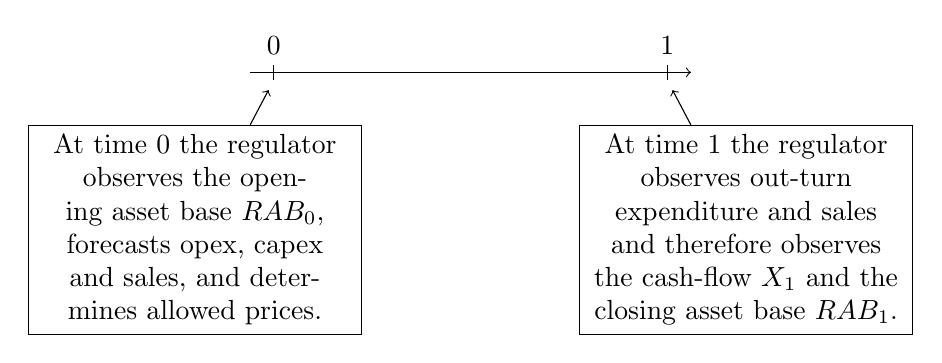
\begin{tikzpicture}
    \draw [->] (-0.3,0) to (5.3,0);
    \draw (0,-0.1) to (0,0.1);
    \draw (5,-0.1) to (5,0.1);
    \node [above] (A) at (0,0.1) {0};
    \node [above] (B) at (5,0.1) {1};
    \node (A1) at (0,-0.1) {};
    \node (B1) at (5,-0.1) {};
    \node [draw, text width=4 cm, align = center] (C) at (-1,-2) {At time 0 the regulator observes the opening asset base $RAB_0$, forecasts opex, capex and sales, and determines allowed prices.};
    %\node [text width=4 cm, align = center] at (2.5,-2) {During the regulatory period the regulated firm incurs expenditure and makes sales at regulated prices.}
    \node [draw, text width=4 cm, align = center] (D) at (6,-2) {At time 1 the regulator observes out-turn expenditure and sales and therefore observes the cash-flow $X_1$ and the closing asset base $RAB_1$.};
    \draw [->] (C) to (A1);
    \draw [->] (D) to (B1);
    \end{tikzpicture}
    \label{fig:1}
\end{figure}

Formally the regulatory process operates as follows: At the start of each regulatory period the regulator chooses the cash-flow of the firm $X_1$ and the closing asset base $RAB_1$ in such a way that the present value of the sum of these two is equal to the opening asset base $RAB_0$:
\begin{equation}
    RAB_0=\V_0(X_1+RAB_1)\label{eqn:bbm}
\end{equation}

 Under these assumptions the Fundamental Theorem of Regulation (see Appendix \ref{app:b}) shows that, at each point in time the asset base is equal to the future stream of cash-flows $RAB_t=\V_t(X_{t+1}, X_{t+2}, \ldots)$ and the regulated firm achieves NPV=0.

We will refer to $X_1$ as the \textbf{one-period cash-flow} of the firm, and the sum $X_1+RAB_1$ as the \textbf{combined cash-flow}.

Equation \ref{eqn:bbm} may look at first abstract, but we can move a step closer to regulatory practice by expanding the present value using the definition of the cost of capital and re-writing the equation as an expression for the allowed level of the cash-flow:
\begin{align}
    RAB_0 &= \V_0(X_1+RAB_1) = \frac{\E_0(X_1+RAB_1)}{\R_{0 \to 1}(X_1+RAB_1)}\nonumber\\
    \implies \; \E_0(X_1) &= \R_{0 \to 1}(X_1+RAB_1) \times RAB_0 -\E_0(RAB_1)\label{eqn:bbm9}
\end{align}

This equation can be made to look more familiar by adopting the conventional definition of the cost of capital $1+r_{0\to t}(X_t)=\R_{0 \to t}(X_t)$ and expanding the cash-flow allowance into its components:
\begin{equation}
X_1 = \underbrace{R_1}_{\text{Revenue}} - \underbrace{O_1}_{\text{Opex}} - \underbrace{K_1}_{\text{Capex}}
\end{equation}
With these definitions, equation \ref{eqn:bbm9} can be written in the following way: The expected revenue allowance\footnote{The revenue $R_1$ here should not be confused with the cost of capital $\R_{0 \to 1}$, for which we will use the blackboard bold font.} can be written as the normal sum of opex, `return on' and `return of' capital:
\begin{equation}
\E_0(R_1) = \underbrace{r_{0 \to 1}(X_1+RAB_1) \times RAB_0}_{\text{`Return on capital'}} + \underbrace{\E_0(O_1)}_{\text{Opex}} + \underbrace{\E_0(Dep_{0 \to 1})}_{\text{`Return of capital'}}\label{eqn:bbm10}
\end{equation}
Here:
\begin{equation}
Dep_{0 \to 1} = RAB_0 + K_1 - RAB_1\label{eqn:bbm11}
\end{equation}
Equations \ref{eqn:bbm10} and \ref{eqn:bbm11} are the familiar two equations which define the Building Block Model (the standard regulatory process used in Australia and around the world).

\subsection*{Problems in the estimation of the cost of capital}

The previous section noted that equation \ref{eqn:bbm9} (or its more familiar variants, equations \ref{eqn:bbm10} and \ref{eqn:bbm11}) captures the standard formulation of the regulatory process. But it is already apparent that there is a problem. As equation \ref{eqn:bbm9} shows, the fundamental task of the regulator is to choose a set of regulated prices so that the value for the expected cash-flow $X_1$ satisfies equation \ref{eqn:bbm9}. But $X_1$ appears on both sides of equation \ref{eqn:bbm9}. The regulator cannot obtain a formally correct cash-flow allowance $\E_0(X_1)$ (or cost of capital $\R_{0 \to 1}(X_1+RAB_1)$) without knowing how the cost of capital depends on the cash-flow allowance.\footnote{A similar circularity problem can arise when estimating the cost of capital using a weighted average formula: the weightings on the cost of equity and the cost of debt depend, in part on the value of the firm, which depends on the cost of capital. See \cite{mohanty2003practical}.}

In addition, the cost of capital $\R_{0 \to 1}(X_1+RAB_1)$ will, in general, depend on the choice of the closing asset base $RAB_1$.\footnote{In cases where the closing asset base is stochastic the cost of capital may also depend on the variation in the closing asset base.} Because the regulatory asset base varies over the life of the firm, we can expect that the cost of capital $\R_{0 \to 1}(X_1+RAB_1)$ also varies over the life of the firm, even if all other factors in the environment remain constant.

The standard resolution of this problem in regulatory practice is just to assume that the cost of capital $\R_{0 \to 1}(X_1+RAB_1)$ is independent of the cash-flow allowance $\E_0(X_1)$ and independent of the choice of the closing asset base $RAB_1$. This is a heuristic which is virtually universal in regulatory practice.

Is there a formulation of the regulatory process which does not suffer from this circularity problem? It turns out that there is. We can see this by returning to equation \ref{eqn:bbm}, and re-writing it as follows:
\begin{align}
    RAB_0 &=\V_0(X_1)+\V_0(RAB_1)\nonumber\\
    &=\frac{\E_0(X_1)}{\R_{0 \to 1}(X_1)}+\frac{\E_0(RAB_1)}{\R_{0 \to 1}(RAB_1)}
\end{align}
Therefore, we can re-formulate the Building Block Model (equation \ref{eqn:bbm9}) in a way which resolves the circularity problem:\footnote{As noted in equation \ref{eqn:scale} the cost-of-capital for the one-period cash-flow $\R_{0 \to 1}(X_1)$ is independent of the level of the expected cash-flow $\E_0(X_1)$.}
\begin{equation}
    \E_0(X_1)= \R_{0 \to 1}(X_1) \times RAB_0 -\E_0(RAB_1) \frac{\R_{0 \to 1}(X_1)}{\R_{0 \to 1}(RAB_1)}\label{eqn:b3}
\end{equation}

Comparing equations \ref{eqn:b3} and \ref{eqn:bbm9} we can see that this version of the Building Block Model is similar to the standard approach  except for the following:
\begin{itemize}
    \item The `return on capital' is defined by multiplying the cost of capital for the one-period cash-flow $\R_{0 \to 1}(X_1)$ (rather than the cost of capital for the combined cash-flow $\R_{0 \to 1}(X_1+RAB_1)$) by the opening asset base; and
    \item In the `return of capital', the closing asset base is scaled by the ratio of the costs-of-capital of the components (i.e., the ratio $\R_{0 \to 1}(X_1)/\R_{0 \to 1}(RAB_1)$.
\end{itemize}

We are now in a position to answer the first two of the questions set out above. Does the cost of capital for a regulated firm vary with the level of the regulatory asset base or the level of the allowed cash-flow?

The answer is as follows: In the conventional historic regulatory practice in Australia, the relevant cost of capital (that is, the multiplier of the asset base in the revenue allowance equation) is the cost of capital for the combined cash-flow $\R_{0 \to 1}(X_1+RAB_1)$. This will, in general vary with both the expected level of the one-period cash-flow $\E_0(X_1)$ and the expected level of the closing asset base $\E_0(RAB_1)$ even if nothing else in the environment changes.

In particular, the cost of capital will depend on the ratio of the level the one-period cash-flow relative to the closing asset base. If this ratio is small, the correct cost of capital is closer to the cost of capital for the closing asset base alone $\R_{0 \to 1}(RAB_1)$ which would normally be expected to be close to the risk-free rate. If this ratio is large, the correct cost of capital is closer to the cost of capital for the one-period cash-flow $\R_{0 \to 1}(X_1)$ which could be very large. As the ratio changes the relevant cost of capital will change, even if there are no other changes in the environment. There are examples of this effect in table \ref{table:1} and figure \ref{fig:2} below.

The dependence of the relevant cost of capital on the level of the cash-flow gives rise to a problem of circularity in the regulatory process. This problem of circularity can be resolved by changing the formulation of the Building Block Model to the formulation set out in equation \ref{eqn:b3} in which the relevant cost of capital is the cost of capital for the one-period cash-flow alone. This cost of capital does not depend on the level of the cash-flow.


\subsection*{Do these concerns make a difference in practice?}

The sections above have identified possible concerns with the conventional approach to setting the cost of capital. But do these issues make a material difference in practice?

To make this assessment let's explore how much the cost of capital of the combined cash-flow $\R_{0 \to 1}(X_1+RAB_1)$ might vary even if the costs of capital on the component cash-flows $\R_{0 \to 1}(X_1)$ and $\R_{0 \to 1}(RAB_1)$ remain unchanged.

Let's suppose that the cost of capital for the cash-flow $X_1$, is say, 20\%, and the cost of capital for the closing asset base $RAB_1$ is, say, 5\%, so $\R_{0 \to 1}(X_1)=1.2$ and $\R_{0 \to 1}(RAB_1)=1.05$. Table \ref{table:1} sets out the cash-flow allowance and the relevant cost of capital under different assumptions about the level of the opening and closing asset base.\footnote{The fourth column in table \ref{table:1} is given by equation \ref{eqn:b3}; the fifth column is given by equation \ref{eqn:wa2}.} As can be seen, the cost of capital for the combined cash-flow $X_1+RAB_1$ varies widely with the level of the asset base, even though there is no change in the underlying systematic risk faced by the firm (that is, no change in $\R_{0 \to 1}(X_1)$ and $\R_{0 \to 1}(RAB_1)$).

\newcommand\Tstrut{\rule{0pt}{2.6ex}}         % = `top' strut
\newcommand\Bstrut{\rule[-0.9ex]{0pt}{0pt}}   % = `bottom' strut

\begin{table}[h!]
\singlespacing
\centering
\caption{The combined cost of capital for a regulated firm $\R_{0 \to 1}(X_1+RAB_1)$ varies with the size of the components even if there is no change in the cost of capital for the components}
\begin{tabular}{|c | c | c | c | c | c |} 
 \hline 
 $RAB_0$ & $\E_0(RAB_1)$ & $\R_{0 \to 1}(X_1)$ & $\R_{0 \to 1}(RAB_1)$ & $\E_0(X_1)$ & $\R_{0 \to 1}(X_1+RAB_1)$ \Tstrut\Bstrut\\
 \hline
 \$1,000 & \$900 & 20\% & 5\% & \$171.83 & 7.14\%\Tstrut\\ 
 \$500 & \$400 & 20\% & 5\% & \$142.86 & 8.57\% \\
 \$1,000 & \$800 & 20\% & 5\% & \$285.71 & 8.57\%\\
 \$400 & \$200 & 20\% & 5\% & \$251.73 & 12.86\% \Bstrut\\ 
 \hline
\end{tabular}
\label{table:1}
\end{table}

Figure \ref{fig:2} presents another way of looking at this question. The left hand graph in figure \ref{fig:2} illustrates the impact on the combined cost of capital $\R_{0 \to 1}(X_1+RAB_1)$ of changes in the allowed regulatory cash-flow $\E_0(X_1)$ holding all other factors constant (here we assume $\E_0(RAB_1)=\$1000$ and  $\R_{0 \to 1}(X_1)=1.2$ and $\R_{0 \to 1}(RAB_1)=1.05$ as before). As can be seen, an increase in the allowed regulatory cash-flow (perhaps due to, say, a reduction in forecast expenditure) results in an increase in the combined cost of capital, even if nothing else changes in the environment.

The right hand graph in figure \ref{fig:2} illustrates how the combined cost of capital varies over the life of a firm with changes in the asset base. This graph illustrates the case of a firm which starts with an opening asset base of \$1000, and lasts five years. The regulated cash-flow allowance is chosen to be constant at $\E_t(X_{t+1})=\$263.97$ each year, ensuring that the closing asset base at the end of the life of the firm is zero ($RAB_5=0$). The regulatory asset base starts at \$1000 and declines to zero over the five years. As can be seen, the combined cost of capital $\R_{t \to t+1}(X_{t+1}+RAB_{t+1})$ increases as the regulatory asset base declines.

In both of these graphs the cost of capital for the one-period cash-flow is fixed at 20\% ($\R_{t \to t+1}(X_{t+1})=1.20$) and the cost of capital for the closing asset base is fixed at 5\% ($\R_{t \to {t+1}}(RAB_{t+1})=1.05$). 

\begin{figure}[ht]
\singlespacing
    \centering
    \caption{Illustration of the dependence of the combined cost of capital $\R_{0 \to 1}(X_1+RAB_1)$ on the level of the allowed cash-flow or the regulatory asset base}
    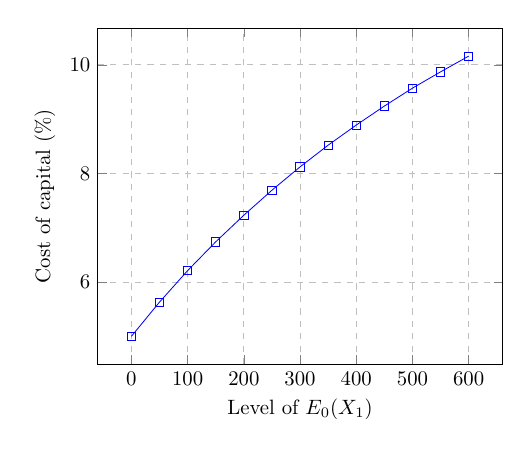
\begin{tikzpicture}[scale=0.75]
        \begin{axis} [
%            title={Temperature dependence of CuSO\(_4\cdot\)5H\(_2\)O solubility},
            xlabel={Level of $\E_0(X_1)$},
            ylabel={Cost of capital (\%)},
%            xmin=0, xmax=100,
%            ymin=0, ymax=120,
%            xtick={0,20,40,60,80,100},
%            ytick={0,20,40,60,80,100,120},
%            legend pos=north west,
            ymajorgrids=true,xmajorgrids=true,
            grid style=dashed,
        ]
        \addplot[
            color=blue,
            mark=square,
            ]
            coordinates {
            (0,5.00)(50,5.63)(100,6.21)(150,6.74)(200,7.23)(250,7.69)(300,8.12)(350,8.52)(400,8.89)(450,9.24)(500,9.57)(550,9.87)(600,10.16)
            };
            %\legend{CuSO\(_4\cdot\)5H\(_2\)O}
        \end{axis}
        \end{tikzpicture}
%
    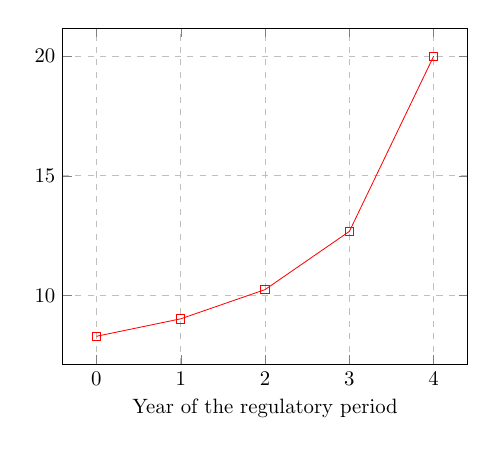
\begin{tikzpicture}[scale=0.75]
        \begin{axis} [
%            title={Temperature dependence of CuSO\(_4\cdot\)5H\(_2\)O solubility},
            xlabel={Year of the regulatory period},
            %ylabel={Cost of capital (\%)},
%            xmin=0, xmax=100,
%            ymin=0, ymax=120,
%            xtick={0,20,40,60,80,100},
%            ytick={0,20,40,60,80,100,120},
%            legend pos=north west,
            ymajorgrids=true,xmajorgrids=true,
            grid style=dashed,
        ]
        \addplot[
            color=red,
            mark=square,
            ]
            coordinates {
            (0,8.3)(1,9.03)(2,10.25)(3,12.68)(4,20)
            };
            %\legend{CuSO\(_4\cdot\)5H\(_2\)O}
        \end{axis}
        \end{tikzpicture}
   \label{fig:2}
\end{figure}




%\subsection*{Resolving the circularity problem}


%What might this mean in practice? Let's consider a simple case in which the opening RAB is $RAB_0=1000$ and the closing RAB is $RAB_1=900$. Let's suppose the cost of capital for the closing RAB (i.e., the risk-free rate), and the expected number of widgets sold is $\E_0(Q_1)=180$. Let's suppose that the risk-free rate is $\R_{0 \to 1}(RAB_1)=1.05$ and the cost of capital for the uncertain volume is $\R_{0 \to 1}(Q_1)=1.26$.\footnote{This is materially larger than the costs of capital that most regulators are familiar with. But this is necessary in this example for the cost of capital for the firm as a whole $\R_{0 \to 1}(R_1+RAB_1)$ to be materially different from the risk-free rate. If the cost of capital for the volume is reduced to, say, $\R_{0 \to 1}(Q_1)=1.10$ (10\%), the cost of capital for the firm as a whole reduces to $\R_{0 \to 1}(R_1+RAB_1)=1.0571$.} Using equation \ref{eqn:b3} the theoretically-correct regulated price is $\bar{P}_1=\$1$ per widget:
%\begin{equation}
%    \bar{P}_1= 1000 \times \frac{1.26}{180}- \frac{900}{180}\times\frac{1.26}{1.05}=1
%\end{equation}

%How different is this to the standard building block model? To apply the standard building block model (equation \ref{eqn:b1}) we need an estimate of the cost of capital for the combined cash-flow $\R_{0 \to 1}(R_1+RAB_1)$. Let's assume that this value is estimated at, say 6\% (perhaps by estimating the cost of capital for a comparator firm). This yields a regulated price of 88.8 cents, materially different from the correct figure.

%Using the values for the costs of capital for $Q_1$ and $RAB_1$, we can use equation \ref{eqn:b2} to determine the correct estimate for the cost of capital of the combined cash-flow $R_1+RAB_1$. This turns out to be 8.00\%, which is quite different to the initial estimate of 6\%.

%To summarise the main result of this section: In order to set a regulated price, the standard application of the building block model (equation \ref{eqn:b1}) requires an estimate of the cost of capital for the combined cash-flow of the regulated firm $\R_{0 \to 1}(X_1+RAB_1)$. But this cost of capital will, in general, depend on the level of the cash-flow $\E_0(X_1)$ which in turn depends on the regulated price. The only way to overcome this problem is to estimate a separate cost of capital for $X_1$ and for $RAB_1$, as in equation \ref{eqn:b3}.


\section{Multi-year regulatory period}\label{sec:rpmy}

For many years, the standard regulatory practice in Australia and New Zealand has involved the use of a fixed-length (five-year) regulatory period, with a single cost of capital for that period. Perhaps unsurprisingly, it turns out that this practice substantially complicates the question of setting the appropriate cost of capital.

%\subsection*{The standard regulatory process when the regulatory period lasts multiple years}

As before, the relevant cost of capital depends very heavily on the precise formulation of the regulatory process. Therefore, as before, we must be precise as to the regulatory process we are using.

Let's suppose that the regulatory period lasts $T$ years (where $T>1$). In the context of a multi-year regulatory period, equation \ref{eqn:bbm} generalises as follows. Given the opening asset base $RAB_0$, the task of the regulator is to choose the cash-flow in each year of the regulatory period $X_1$, $X_2$, \ldots, $X_T$, and the closing asset base $RAB_T$, to satisfy the following expression:
\begin{equation}
    RAB_0=\V_0(X_1, X_2, \ldots, X_T+RAB_T)=\sum_{t=1}^T \V_0(X_t)+\V_0(RAB_T)\label{eqn:c1}
\end{equation}

In common regulatory practice, this is usually implemented as follows. A single parameter, which we will label $R$ is chosen. In addition, a sequence of values of the asset base $RAB_t$ is chosen. The regulated cash-flow allowance in each year of the regulatory period is then determined using a simple analogy to equation \ref{eqn:bbm9}:
\begin{align}
    \forall t=1, \ldots, T,\;\; \E_0(X_t) &=  R \times RAB_{t-1} -\E_0(RAB_t)\label{eqn:c2}
\end{align}

But, how should we choose the parameter $R$? Expanding out equations \ref{eqn:c2} and applying equation \ref{eqn:c1} we find that, given the expected cash-flows $\E_0(X_t)$ and the opening asset base $RAB_0$ and the expected closing asset base $\E_0(RAB_T)$, the parameter $R$ must be chosen to satisfy the following:
\begin{align}
    &\frac{\E_0(X_1)}{R}+\frac{\E_0(X_2)}{R^2}+\ldots+\frac{\E_0(X_T+RAB_T)}{R^T}=RAB_0\label{eqn:c4}
\end{align}
In other words, in this approach to regulation, the correct value for the cost of capital parameter $R$ is the \textbf{internal rate of return} of the cash-flow stream consisting of an outlay of $RAB_0$ at time zero, and cash-flow of $\E_0(X_1), \E_0(X_2), \ldots, \E_0(X_T+RAB_T)$ in the subsequent years of the regulatory period.

But again, we can see that there is a problem. As equation \ref{eqn:c4} makes clear, the parameter $R$ depends on the levels of the individual cash-flows $\E_0(X_1)$, $\E_0(X_2)$ and so on, in a complicated manner. But the parameter $R$ is also a key input into the determination of the $\E_0(X_1)$ and so on through equation \ref{eqn:c1}. Once again we have a problem of circularity.

%\subsection*{Resolving the circularity problem}

As before, this problem can be resolved by changing the regulatory process. Rather than using a single cost of capital parameter $R$ for the entire regulatory period we should use different costs of capital for the individual components of the cash-flow of the firm.

There are two ways that this might be carried out. In the first approach, the allowed cash-flows are all set in advance, based on the costs of capital prevailing at the start of the regulatory period. In the second approach, the allowed cash-flows are set each year of the regulatory period, on the basis of the costs of capital prevailing at that time.

Let's consider the first approach in which the allowed cash-flows are all set in advance. Specifically, let's suppose that the regulator chooses parameters $R_t$ and $S_t$ for $t=1, \ldots, T$. The regulator then sets the cash-flow allowance as follows (this equation is the analogy to equation \ref{eqn:b3}):
\begin{align}
    \forall t=1, \ldots, T,\;\; \E_0(X_t) &=  R_t \times \E_0(RAB_{t-1}) -\E_0(RAB_t)\frac{R_t}{S_t}\label{eqn:d3}
\end{align}
The cash-flows set in this way satisfy the fundamental requirement of equation \ref{eqn:c1} provided we choose $R_1=\R_{0 \to 1}(X_1)$, $S_1 R_2=\R_{0 \to 2}(X_2)$, \ldots , $S_1 S_2 \ldots S_T = \R_{0 \to T}(RAB_T)$. These equations can be satisfied in different ways. However, a straightforward approach is to choose:\footnote{$S_t$ here is the `forward rate' for the cost of capital for the asset base -- specifically, it is the rate at time zero that is forecast to apply between time $t-1$ and time $t$.}
\begin{align}
    R_t &= \frac{R_{0 \to t}(X_t)}{\R_{0 \to {t-1}}(RAB_{t-1})}\label{eqn:rt}\\
    \text{and} \; S_t&=\frac{\R_{0 \to t}(RAB_t)}{\R_{0 \to {t-1}}(RAB_{t-1})}\label{eqn:st}
\end{align}
It is straightforward to check that, with this choice of the parameters, equation \ref{eqn:c1} is satisfied.

Under the second approach, the allowed cash-flows are not fixed in advance, but are set at the start of each year (within the regulatory period) on the basis of information that is available at the time. In this case, the relevant equation for establishing the cash-flow allowance can be written as follows:
\begin{align}
    \forall t=1, \ldots, T,\;\; \E_{t-1}(X_t) &=  R_t \times RAB_{t-1} -\E_{t-1}(RAB_t)\frac{R_t}{S_t}\label{eqn:d4}
\end{align}
This equation is the generalisation of equation \ref{eqn:b3}. The formulae to calculate the relevant values of the parameters $R_t$ and $S_t$ in this case are derived in appendix \ref{app:c}.


To see how the first approach might work in a simple example, let's suppose that we have a regulatory period that lasts five years. At time zero the opening asset base is $RAB_0=\$1,000$. The regulator chooses a path for the asset base $RAB_1=\$900$, $RAB_2=\$800$, \ldots, $RAB_5=\$500$. The cost of capital for the cash-flow and for the asset base (which is just equal to the risk-free rate of 5\% per annum) are set out in table \ref{table:3}. The cost of capital for the asset base (assuming a flat term structure and a risk-free rate of 5\% per annum) is:
\begin{equation}
    \R_{0 \to t}(RAB_t) = (1.05)^t
\end{equation}
The cost of capital for the cash-flow is chosen to satisfy the condition:\footnote{This can be justified using the assumptions that the term structure is flat and no new information about the future cash-flow arrives over time.}
\begin{equation}
    \R_{0 \to t}(X_t) = (1.05)^{t-1}(1.20)
\end{equation}
The remainder of the table shows the implied values of $R_t$ and $S_t$ and the resulting cash-flow allowance $\E_0(X_t)$.\footnote{$R_t$ and $S_t$ are given by equations \ref{eqn:rt} and \ref{eqn:st} respectively. $\E_0(X_t)$ is given by equation \ref{eqn:d3}.}

Using these values we can calculate that the value of the parameter $R$ (the single cost of capital for entire regulatory period) is 7.16\%. As before, this value is a complicated mix of the different costs of capital for the different cash-flows and timings during the regulatory period. It is not possible to calculate this value until after the regulatory cash-flow allowances have been determined.

The last row of table \ref{table:3} shows the implied value for the cost of capital that would be required if the regulator followed the naive approach of equation \ref{eqn:bbm9}. As can be seen, in this case the parameter chosen is a `mixture' of cost of capital for the cash-flow $X_t$ and the asset base $RAB_t$ and varies across the regulatory period.

\begin{table}[h!]
\singlespacing
\centering
\caption{Illustration of calculating the cash-flow allowance over a five-year regulatory period}
\begin{tabular}{|c | c | c | c | c | c | c |} 
 \hline
 Time & $t=0$ & $t=1$ & $t=2$ & $t=3$ & $t=4$ & $t=5$\Tstrut\Bstrut\\ 
 \hline
 $RAB_t$ & \$1,000 & \$900 & \$800 & \$700 & \$600 & \$500\Tstrut\\ 
 $\R_{0 \to t}(X_t)$ & 1.000 & 1.200 & 1.260 & 1.323 & 1.389 & 1.459 \\
 $\R_{0 \to t}(RAB_t)$ & 1.000 & 1.05 & 1.103 & 1.158 & 1.216 & 1.276 \\
 $R_t$ &  & 1.20 & 1.20 & 1.20 & 1.20 & 1.20\\
 $S_t$ &  & 1.05 & 1.05 & 1.05 & 1.05 & 1.05\\
 $\E_0(X_t)$ & & \$171.43 & \$165.71 & \$160.00 & \$154.29 & \$148.57 \\
 Implied CoC & & 7.14\% & 7.30\% & 7.50\% & 7.76\% & 8.10\% \Bstrut\\ 
 \hline
\end{tabular}
\label{table:3}
\end{table}

At this point we can answer one of the questions posed at the outset: What is the correct term for the cost of capital used in regulatory proceedings? From the analysis above we can provide the following answer:
\begin{itemize}
    \item Where a single cost-of-capital parameter is used to determine all of the cash-flow allowances throughout a regulatory period (as in equation \ref{eqn:c2}), there is no single correct `term' for this cost-of-capital. Rather, this cost of capital is a mix of a number of different terms (corresponding to the cash-flows within the regulatory period, and the asset base at the end of the regulatory period). The term of each of these individual cash-flows is shorter than or equal to the length of the regulatory period. Formally it is the internal rate of return associated with a cash-flow stream.
    \item As before there arises a circularity problem. The single cost-of-capital parameter depends on the cash-flow allowances, but the cash-flow allowances depend on this cost-of-capital parameter. In order to resolve the circularity problem we must use a separate cost of capital for each of the individual components of the cash-flow of the firm -- that is, a separate cost of capital for $X_t$, $t=1, \ldots, T$ and $RAB_T$.
    
    In the case where all of the cash-flow allowances are set at the beginning of the period (the first approach above), the regulatory process must follow equation \ref{eqn:d3}. Specifically:
    \begin{itemize}
        \item The relevant cost of capital for the purposes of determining the allowed `return on capital' (that is, the coefficient on the regulatory asset base) must be given by:
        \begin{equation}
            R_t=\frac{R_{0 \to t}(X_t)}{\R_{0 \to {t-1}}(RAB_{t-1})}
        \end{equation}
        \item In calculating the `return of capital' the closing regulatory asset base must be scaled by
        \begin{equation}
            \frac{R_t}{S_t}=\frac{R_{0 \to t}(X_t)}{\R_{0 \to {t}}(RAB_t)}
        \end{equation}
        This reduces to equation \ref{eqn:b3} in the case of a regulatory period of one year.
    \end{itemize}
    
\end{itemize}


As an illustration of the effect of these observations, let's use some typical values for the cash-flow and asset base drawn from an actual regulatory proceeding. In this case we will use distribution businesses in Australia. These are regulated using a five-year regulatory cycle. From the discussion above, this means that there are 6 costs-of-capital we need to estimate: $\mathbb{R}_{0 \to t}(X_t)$, $t=1,\ldots,5$ and $\mathbb{R}_{0 \to 5}(RAB_5)$. We will assume values for these costs of capital and then determine the implications for the value of the parameter $R$.

As before we will assume that the (annualised) risk-free interest rate for all terms is, say, 1.05 (5\%). In other words, the cost of capital for a fixed value in one year is $1.05$, in two years is $1.05^2$, and so on. Following standard regulatory practice, we will make the assumption that $RAB_5$ is a fixed number, so it should receive a cost of capital equal to the risk-free rate which as just noted, is $1.05^5$. We will make the assumption that, at time 0, $\mathbb{V}_{s \to t}(X_t)$ is a fixed value for $0<s<t$.\footnote{In essence, this assumes that the regulator receives no new information about the future cash-flows until the year in which the cash-flow is received.} Finally, we will assume that $\mathbb{V}_{t-1 \to t}(X_t) = \mathbb{E}_{t-1}(X_t) / 1.35$. It follows that the cost of capital for the first cash-flow $X_1$ is 1.35 (as before), and for all the other cash-flows:
\begin{equation}
    \mathbb{R}_{0 \to t}(X_t) = (1.05)^{t-1}(1.35)
\end{equation}

Given these assumed values for the component costs of capital, we can use the actual cash-flow and closing asset base for the 13 electricity network distribution businesses on the east coast of Australia (known as Distribution Network Service Providers, or DNSPs) over the period 2014-2019 to determine the value of $R$ which satisfies equation \ref{eqn:c4}. The results are set out in table \ref{table:3}. As can be seen, the variation in the relative size of the cash-flows gives rise to a variation of about 400 basis points in the discount factor $R$, even though all of these DNSPs are assumed to have exactly the same underlying component costs of capital. This variation is roughly the same size as a variation in, say, the market risk premium of 0.5\%. 

\begin{table}[h!]
\singlespacing
\centering
\caption{Illustration of different values of the discount factor $R$ for real-world distribution network businesses with the same underlying component costs of capital}
\begin{tabular}{|c | c |} 
 \hline
 DNSP & Value of $R$ \Tstrut\Bstrut\\
 \hline
 Energex & 5.543\% \Tstrut\\ 
 Evoenergy & 5.581\% \\
 AusNet & 5.622\% \\
 Ergon Energy & 5.631\% \\
 CitiPower & 5.649\% \\
 United Energy & 5.688\% \\
 Powercor & 5.735\% \\
 Jemena & 5.753\% \\
 Ausgrid & 5.819\% \\
 Endeavour Energy & 5.796\% \\
 TasNetworks & 5.920\% \\
 SA Power Networks & 5.922\% \\
 Essential Energy & 5.942\%
 \Bstrut\\ 
 \hline
\end{tabular}
\label{table:3}
\end{table}


\section{The cost of capital for the debt stream}\label{sec:cod}

In standard regulatory practice the relevant cost of capital for regulatory purposes is often estimated as a weighted average of the cost of capital for the debt and equity cash-flow streams of the regulated firm.\footnote{In conventional corporate finance theory and practice, it is common to observe that the total cash-flow of the firm (denoted $X_1$, $X_2$, \ldots above) is paid out to the investors in the form of two distinct streams of payments: The payments to equity holders (in the form of dividends, plus share buybacks, less new share issues), and the payments to debt holders (in the form of interest payments, plus retirement of existing debt, less new debt issues). It is common to seek to estimate the cost of capital for the equity payment stream and the debt payment stream separately, before recombining them to find the `weighted average' cost of capital for the firm as a whole.} In addition, in standard regulatory practice the cost of capital for debt is typically estimated as the current `yield to maturity' on a corporate bond of the relevant credit rating and term. Usually the term is taken to be the same as the length of the regulatory period (e.g., five years) or longer (say, ten years). In recent years some regulators in Australia have used a cost of debt which is based on a trailing average of historic rates on corporate bonds of the relevant credit rating and term.

What can we say about the theoretically-correct approach to estimating the cost of debt in regulatory proceedings?

%This may make sense if the cost of capital for the debt stream is easier to estimate than the cost of capital for the firm as a whole. This would be the case, for example, if the relevant cost of capital could be inferred from the observed prices of traded debt instruments. On the face of it, this is not an unreasonable hope -- there are many actively traded debt instruments whose observed prices shed some light on the associated cost of capital. Provided we take into account the term and credit rating, these debt instruments will often be a close substitutes for the debt instruments of the regulated firm whose cost of capital we are trying to estimate. But can we use the observed prices of these debt instruments to estimate the cost of debt for regulatory purposes?

%But what, exactly, is the right regulatory allowance for the cost of capital of the debt stream? Perhaps unsurprisingly, given the analysis above, the answer depends, critically, on how the regulatory process is carried out. We will discuss several possibilities below.

\subsection*{Debt preliminaries}

let's assume that we have a set of debt instruments, distinguished only in their date of maturity $t$.\footnote{All other characteristics of the debt instruments, such as the credit rating, or seniority, are assumed to be chosen so that the traded debt instruments are a perfect substitute for the debt instruments of the firm whose cost of capital we are estimating.}
The debt instrument which matures at time $t$ is assumed to make an uncertain payoff given by the random variable $I_t$ at time $t$. There are no other payments from each debt instrument (i.e., they are `zero coupon bonds').\footnote{This is without loss of generality as a regular bond paying coupons can be constructed out of a series of zero-coupon bonds.} These instruments are assumed to be actively traded in an efficient market. The current price of this debt instrument in the market is its present value $\mathbb{V}_{0 \to t}(I_t)$. It follows that the cost of capital to maturity of each of these instruments is the ratio of the expected future payoff $\mathbb{E}_0(I_t)$ to the current market price $\mathbb{V}_{0 \to t}(I_t)$:
\begin{equation}
    \mathbb{R}_{0 \to t}(I_t)=\frac{\mathbb{E}_0(I_t)}{\mathbb{V}_{0 \to t}(I_t)}
\end{equation}


At time zero the regulated firm is assumed to hold a portfolio of debt instruments, with a volume of the instrument maturing at time $t$ given by the quantity $D_{0 \to t}$ for $t=1,2, \ldots$. From the linearity of the value function, the value of this portfolio at time zero can be directly derived from the current observed price of each debt instrument:
\begin{equation}
    \sum_{t=1} \mathbb{V}_{0\to t}(D_{0 \to t}I_t) = \sum_{t=1} D_{0 \to t} \mathbb{V}_{0\to t}(I_t) 
\end{equation}

At the end of the first period, the debt instrument maturing at time $t=1$ matures, making the payoff $D_{0 \to 1} I_1$. In addition, at this time the firm is assumed to be able to make changes to its portfolio of debt instruments. We can represent this by the assumption that the firm sells its entire portfolio purchased at time zero, which has the value at time 1 of $\sum_{t=2} \mathbb{V}_{1\to t}(D_{0 \to t}I_t)$, and then purchases a new portfolio of debt instruments, given by the quantity $D_{1 \to t}$ of the instrument $I_t$, $t=2,3 , \ldots$. The cost of purchasing this new portfolio (which is also its current value) is $\sum_{t=2} \mathbb{V}_{1\to t}(D_{1 \to t}I_t)$. Ignoring transactions costs, the net payoff at time one is therefore as follows:
\begin{equation}
    X^D_1=D_{0 \to 1} I_1 + \sum_{t=2} D_{0 \to t} \mathbb{V}_{1\to t}(I_t) - \sum_{t=2} D_{1 \to t} \mathbb{V}_{1\to t}(I_t)\label{eqn:dps1}
\end{equation}
The combined payoff is therefore:
\begin{equation}
    X^D_1+\V^D_1=D_{0 \to 1} I_1 + \sum_{t=2} D_{0 \to t} \mathbb{V}_{1\to t}(I_t)\label{eqn:dps2}
\end{equation}

Importantly, the present value of the stream of debt payments at time zero depends \textit{only} on the value of the debt portfolio that is held at time zero (all future changes in the debt portfolio are of no consequence). This is demonstrated in appendix \ref{app:d}. 

\subsection*{Estimating the cost of debt in a one-year regulatory period}



%Although it is always true that we can decompose the cash-flow of the firm into payments to equity and payments to debt, as in equation \ref{eqn:decomp}, if the firm can adjust its debt portfolio over time, we usually will not be able to estimate the cost of capital for the cash-flow to debt $X^D_1$ separately from the cost of capital for the remaining value $\V^D_1$.  If we assume that the firm retains discretion to change its debt portfolio at each time period, at time zero we can estimate the cost of debt for the cash-flow $X^D_1+\mathbb{V}^D_1$ but not $X^D_1$ and $\mathbb{V}^D_1$ separately.

%The same is true for a sequence of cash-flows. If we assume that the firm has discretion to change its debt portfolio each period, at time zero we cannot estimate a cost of debt for the debt payment stream $X^D_1, X^D_2+ \mathbb{V}^D_2$, as these values $X^D_1$ and $X^D_2+ \mathbb{V}^D_2$ depend on the choice of the debt portfolio at time 1. If we are to estimate the cost of debt for $X^D_1$ and $\mathbb{V}^D_1$ separately, or for a debt payment stream $X^D_1, X^D_2+ \mathbb{V}^D_2$ we must make the assumption that the changes in the debt portfolio are pre-determined (`locked in') at the outset (at time zero). In our view this assumption is unrealistic, but we will need to maintain this assumption to derive the results below.

%We will make the assumption that the debt payment stream is determined by the payments on maturing debt plus any changes in the debt portfolio, as given in equation \ref{eqn:dps1}. The regulatory process will focus on determining the stream of payments to equity $(X^E_1, X^E_2, \ldots)$, which we will define as $X^E_t=X_t-X^D_t$.

Let's assume that the stream of payments to equityholders and debtholders are denoted $(X^E_1, X^E_2, \ldots)$ and $(X^D_1, X^D_2, \ldots)$, respectively. The total cash-flow of the firm is assumed to be paid out in total to equityholders and debtholders each period:
\begin{equation}
    \forall t, \; X_t=X^E_t+X^D_t\label{eqn:decomp}
\end{equation}
As above, the cash-flow stream to debtholders $X^D_t$ is determined by the portfolio of debt instruments held by the firm (that is, any payments for maturing debt instruments) plus purchases of new debt instruments less sales of old debt instruments.


Let's return now to the case of a one-year regulatory period. As we have seen, the standard regulatory practice involves estimating a single cost of capital for the firm as a whole $X_1+RAB_1$, which we labeled $\R_{0 \to 1}(X_1+RAB_1)$. 
%
It follows immediately from equation \ref{eqn:decomp} that the cost of capital for the combined cash-flow of the firm $\R_{0 \to 1}(X_1+RAB_1)$ can be expressed as a weighted average of the cost of capital for the equity payment stream $\R_{0 \to 1}(X^E_1+\V^E_1)$ and the cost of capital for the debt payment stream $\R_{0 \to 1}(X^D_1+\V^D_1)$, using either of the weighted average formulae in equations \ref{eqn:wa1} or \ref{eqn:wa2}.
%
Let's put aside the circularity problems discussed above and explore what we can say about the estimation of the cost of debt as a step toward the estimation of the cost-of-capital for the firm as a whole.

The relevant cost of debt is the cost of capital for the combined debt cash-flow  $X^D_1+\mathbb{V}^D_1$. We can express this cost of debt as the weighted average of the cost of capital of the instruments in the portfolio:
    \begin{align}
    \R_{0 \to 1}(X^D_1+\V^D_1) &= \frac{\E_0(X^D_1+\V^D_1)}{\V_{0 \to 1}(X^D_1+\V^D_1}\nonumber\\
    &=D_{0 \to 1}\frac{\E_0(I_1)}{\V^D_0}+ \sum_{t=2} D_{0 \to t} \frac{\E_0(\V_{1 \to t}(I_t))}{\V^D_0}\nonumber\\
    &=D_{0 \to 1}R_{0 \to 1}(I_1)\frac{\V_{0 \to 1}(I_1)}{\V^D_0}\nonumber\\
    &+\sum_{t=2} D_{0 \to t} \R_{0 \to 1}(\V_{1\to t}(I_t))\frac{\V_{0 \to t}(I_t)}{\V^D_0}\label{eqn:dcoc}
    \end{align}

    The weighting on each instrument in this depends on the ratio of the current price for the debt instrument in the market  $\V_{0\to t}(I_t)$ to the total value of the portfolio  $\V_0^D$. In principle both of these can be easily observed. In addition, the relevant cost of capital for the one-year debt instrument $I_1$ can, is the ratio of the expected payoff in one year $\E_0(I_1)$ to the current market price $\V_0(I_1)$:
    \begin{equation}
        \R_{0 \to 1}(I_1) = \frac{\E_0(I_1)}{\V_0(I_1)}
    \end{equation}
    In principle the expected payoff on the debt instrument can be estimated if we can estimate the probability of default and the likely recovery of funds to debtholders in the event of default. As noted above, the current market price can be easily observed. As a consequence, the relevant cost of capital for a one-year debt instrument can, in principle be estimated.

    But what about the relevant cost of capital for the longer-term debt instruments in the portfolio? For longer-term debt instruments the relevant cost of capital for each instrument in equation \ref{eqn:dcoc} is the cost of capital associated with holding the long-term debt instrument from time zero to time one: $\R_{0 \to 1}(\V_{1\to t}(I_t))$. This is equal to the expected future (time one) price of the instrument over the current price:
    \begin{equation}
        \R_{0 \to 1}(\V_{1 \to t}(I_t)) = \frac{\E_0(\V_{1 \to t}(I_t))}{\V_{0 \to 1}(\V_{1 \to t}(I_t))}=\frac{\E_0(\V_{1 \to t}(I_t))}{\V_{0 \to t}(I_t)}
    \end{equation}

Unfortunately, the expected future price of the debt instrument $\E_0(\V_{1 \to t}(I_t))$ cannot be easily observed in the market. This value is related to forecasts of future interest rates and investor tolerance of risk.

These observations are illustrated in figure \ref{fig:3}. Let's assume that the regulated firm holds a portfolio of debt instruments maturing in one, two and three years, labelled $I_1$, $I_2$, and $I_3$. Each of these instruments has a `face value' of, say, \$1000. The current price of these three instruments is \$900, \$800, and \$700, say. The regulator can in principle estimate the expected payout on the instrument maturing in one year, $I_1$. Although it has a face value of \$1000, the actual expected payout will be somewhat less, reflecting the probability of default and the recovery expected in the event of default. Let's suppose that the expected future payout is, say, \$950. In this case the cost of capital for this instrument is $\$950/\$900-1 = 5.56\%$. But in the case of the longer-term instruments $I_2$ and $I_3$ it is not easy to estimate the price of these instruments at time one. As a result estimating the cost of capital between time 0 and time 1 for these instruments is not straightforward.

\begin{figure}[ht]
\singlespacing
    \centering
    \caption{It is not, in general, possible to estimate the cost of capital for a portfolio of debt instruments using currently observed market data}
    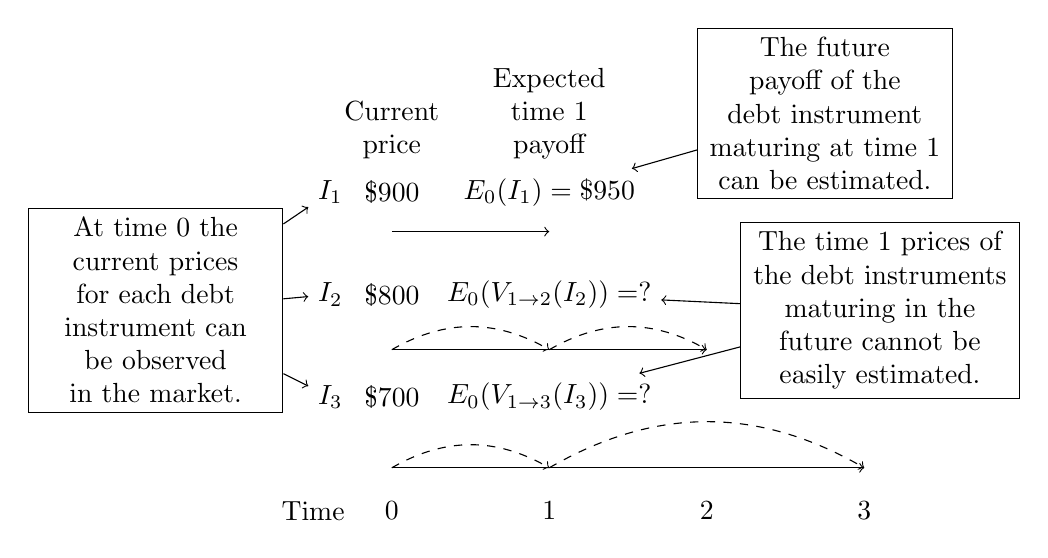
\begin{tikzpicture}
    \draw [->] (0,2.5) to (2,2.5);
    \draw [->] (0,1) to (4,1);
    \draw [->] (0,-0.5) to (6,-0.5);
    \draw [->,dashed, bend left] (0,1) to (2,1);
    \draw [->,dashed, bend left] (0,-0.5) to (2,-0.5);
    \draw [->,dashed, bend left] (2,1) to (4,1);
    \draw [->,dashed, bend left] (2,-0.5) to (6,-0.5);
    %\draw [dashed] (4,-0.2) to (4,4.2);
    %\draw [dashed] (6,-0.2) to (6,4.2);
    \node [below] at (-1,-0.8) {Time};
    \node [below] (A) at (0,-0.8) {0};
    \node [below] (B) at (2,-0.8) {1};
    \node [below] (C) at (4,-0.8) {2};
    \node [below] (C1) at (6,-0.8) {3};
    \node [above, text width =1.5 cm, align =center] (D) at (0,3.3) {Current price};
    \node [above, text width =1.5 cm, align =center] (E) at (2,3.3) {Expected time 1 payoff};
    \node [left] (I1) at (-0.5,3) {$I_1$};
    \node [left] (I2) at (-0.5,1.7) {$I_2$};
    \node [left] (I3) at (-0.5,0.4) {$I_3$};
    \node  (F1) at (0,3) {\$900};
    \node  (G1) at (0,1.7) {\$800};
    \node  (H1) at (0,0.4) {\$700};
    \node (L1) at (2,3) {$\E_0(I_1)=\$950$};
    \node (L2) at (2,1.7) {$\E_0(\V_{1 \to 2}(I_2))=?$};
    \node (L3) at (2,0.4) {$\E_0(\V_{1 \to 3}(I_3))=?$};
    \node [draw, text width=3 cm, align = center] (box1) at (-3,1.5) {At time 0 the current prices for each debt instrument can be observed in the market.};
    \node [draw, text width=3 cm, align = center] (box2) at (5.5,4) {The future payoff of the debt instrument maturing at time 1 can be estimated.};
    \node [draw, text width=3.3 cm, align = center] (box3) at (6.2,1.5) {The time 1 prices of the debt instruments maturing in the future cannot be easily estimated.};
    \draw [->] (box1) to (I1);
    \draw [->] (box1) to (I2);
    \draw [->] (box1) to (I3);
    \draw [->] (box2) to (L1);
    \draw [->] (box3) to (L2);
    \draw [->] (box3) to (L3);
    \end{tikzpicture}
    \label{fig:3}
\end{figure}

We are now in a position to answer one of the questions asked at the outset: Can we estimate the cost of debt for a regulated firm by observing the appropriate yield-to-maturity on a corporate bond of the right term? If so, what is the right term?

This analysis provides no support for the assertion that, in standard regulatory practice, we can estimate the cost of debt for a regulated firm by observing the yield-to-maturity on a corporate bond of the right term, for the following reasons:
\begin{itemize}
    \item In standard, historic regulatory practice (as summarised in equation \ref{eqn:bbm9} or equations \ref{eqn:bbm10} and \ref{eqn:bbm11}), the regulator is interested in estimating the cost of capital of the combined cash-flow for the firm as a whole. If we seek to estimate this cost of capital as a weighted average of the cost of equity and the cost of debt the relevant cost of capital for debt is the cost of capital for the debt payment stream of the firm. $\R_{0 \to 1}(X^D_1+\V^D_1)$. This depends on the \textit{portfolio of debt instruments} held by the regulated firm (and not just the cost of capital for a single bond).

    \item In general, the debt portfolio held by the regulated firm will include instruments with a range of terms. Although it is relatively easily to estimate the cost of capital for a debt instrument maturing in one year, it is not straightforward to estimate the one-year cost of capital for debt instruments maturing in future years.

    \item The current yield-to-maturity of a debt instrument is the ratio of the `face value' to the current price. But the relevant cost of capital $\R_{0 \to t}(I_t)$ is the ratio of the expected future payout to the current price:
    \begin{equation}
        \R_{0 \to t}(I_t)=\frac{\E_0(I_t)}{\V_{0 \to t}(I_t)}
    \end{equation}
    For any debt instrument other than a risk-free instrument, the expected future payout $\E_0(I_t)$ is less than the face value due to the probability of default. Therefore, the yield-to-maturity on a bond is an over-estimate of the cost of capital for that bond.
\end{itemize}

If the cost of capital for the debt portfolio of the regulated firm cannot be easily observed (as appears to be normally assumed) it follows that there appears to be little value in separating the cost of capital for the firm as a whole into a weighted average of the cost of equity and the cost of debt.

This leaves two possibilities: We could estimate the cost of capital for the firm as a whole (as before) -- or, more strictly, the component costs of capital for the firm as a whole, as set out in equation \ref{eqn:b3}. Alternatively, we could implement a version of the regulatory process which only requires estimation of the (components of the) costs of equity.

To see how this might be achieved, let's assume that the cash-flow stream to debt can be treated as exogenous -- determined outside the regulatory process. The regulatory process then determines the equity cash-flow $X^E_1$ and the equity asset base $RAB^E_1$. The required version of the Building Block Model equations can be derived as follows. First, equation \ref{eqb:bbm} can be expanded as follows:
\begin{align}
    RAB_0 &= \V_{0}(X_1+RAB_1) = \V_{0}(X^E_1+RAB^E_1 + X^D_1+\V^D_1)\nonumber\\
    &= \frac{\E_{0}(X^E_1)}{\R_{0 \to 1}(X^E_1)}+\frac{\E_{0}(RAB^E_1)}{\R_{0 \to 1}(RAB^E_1)} + \V_{0 \to 1}(X^D_1+\V^D_1)
\end{align}
It follows that the allowed cash-flow stream to equity of the regulated firm should be determined as follows:
\begin{align}
    \E_0(X^E_1) &= RAB_0 \times \R_{0 \to 1}(X^E_1) 
    - \E_{0}(RAB^E_1) \frac{\R_{0 \to 1}(X^E_1)}{\R_{0 \to 1}(RAB^E_1}\nonumber\\
    &+ \V_{0 \to 1}(X^D_1+\V^D_1) \R_{0 \to 1}(X^E_1)\nonumber\\
    &=RAB_0 \times \R_{0 \to 1}(X^E_1)  \nonumber\\
    &- \left(\E_{0}(RAB^E_1)- \R_{0 \to 1}(RAB^E_1) \sum_{t=1} D_{0 \to t} \V_{0 \to t}(I_t)\right)\frac{\R_{0 \to 1}(X^E_1)}{\R_{0 \to 1}(RAB^E_1)}\label{eqn:f1}
\end{align}

This is a further variation on the Building Block Model, extending equation \ref{eqn:b3} by replacing the expected closing asset base $\E_{0}(RAB^E_1)$ with an expression that subtracts the current value of the debt portfolio: $\E_{0}(RAB^E_1)- \R_{0 \to 1}(RAB^E_1) \sum_{t=1} D_{0 \to t} \V_{0 \to t}(I_t)$. This last term ($\sum_{t=1} D_{0 \to t} \V_{0 \to t}(I_t)$) can be directly observed from market data.





%[How should we then proceed with the estimation of the cost of capital for regulatory purposes? Is there any value in seeking to estimate a different cost of capital for debt and for equity? The analysis here calls this practice into question. As we have seen, the relevant costs of capital that we require for regulatory purposes is the cost of capital for the cash-flow $\R_{0 \to 1}(X_1)$ and for the closing asset base $\R_{0 \to 1}(RAB_1)$. It is not clear that there is any value at all in decomposing the cash-flow $X_1$ into payments to equity and payments to debt $X_1=X^E_1+X^D_1$. As we have seen, the cash-flow to debt $X_D^1$ depends on the change in the debt position from one period to the next. It is not possible to determine a cost of capital for this value (as it depends on the future actions of the firm). As we have seen, even if we sought to obtain a cost of capital for the combined payments on the debt portfolio $X^D_1+\V^D_1$, this value cannot be directly observed from market data.

%This analysis calls into question the use of a separate cost of equity and cost of debt in regulatory proceedings.]

We have seen that, in the case of a single-year regulatory period, if we use a single cost of capital for the combined cash-flow of the firm it is possible to write that cost of capital as a weighted average of the (combined) cost of capital for debt and the (combined) cost of capital for equity. If we seek to implement a version of the regulatory process in which we estimate separate costs of capital for the components (as in equation \ref{eqn:b3}) then again we can express the costs of capital for those components as a weighted average of the corresponding component cost of capital for debt and equity separately.

What about the case of a multi-year regulatory period? Let's suppose that we seek to estimate a single cost of capital for the entire regulatory period (as in equation \ref{eqn:c2}. Can we express this cost of capital parameter $R$ as a weighted average of the corresponding parameter for equity and for debt?

The answer is no. Let's suppose that the parameter $R$ satisfies equation \ref{eqn:c4} and the corresponding parameter $R^E$ and $R^D$ satisfies the corresponding equation for debt and equity. In the case where $T=2$ this yields the following:
\begin{align}
    &\frac{\E_0(X_1)}{R}+\frac{\E_0(X_2+RAB_3)}{R^2}\nonumber\\
    &=\frac{\E_0(X^E_1)}{R^E}+\frac{\E_0(X^E_2+RAB^E_2)}{{R^E}^2}+\frac{\E_0(X^D_1)}{R^D}+\frac{\E_0(X^D_2+\V^D_2)}{{R^D}^2}
\end{align}
In this case the parameter $R$ cannot be expressed as a weighted average of $R^D$ and $R^E$. This calls into question the common use of a weighted-average cost of capital in the context of a multi-year regulatory period.


%\subsection*{The cost of debt with a regulatory period of $T$ years}

%Let's now continue to extend the analysis to the case of a regulatory period of several years. One possible approach, as we have seen earlier, is to adopt a regulatory process which determines the cash-flow $X_1$ and the asset base $RAB_1$ for the firm as a whole. As we have seen, as part of this process the regulator must determine the parameters $A_{0\to 1}, A_{0 \to 2}, \ldots, A_{0 \to T}$ and $B_{0 \to T}$. The equations for this approach are set out earlier in equations \ref{eqn:basicbbm2a}, \ref{eqn:basicbbm2b} and \ref{eqn:basicconden}.

%In the case where these parameters are all chosen separately, each parameter is the weighted average of the corresponding components for equity and debt, in a straightforward generalisation of equations X and Y. We can also choose all of these parameters to be equal to a common value, in which case the parameters must be set equal to a weighted average of all of the components, in a straightforward generalisation of equation Z.

%But, as we have noted earlier, this is not how regulation is usually carried out. As we have seen, the most common approach involves setting these parameters as follows: $A_{0 \to 1}=R$, $A_{0 \to 2}=R^2$, $A_{0 \to T-1}=R^{T-1}$, $A_{0 \to T}=B_{0 \to T}=R^T$. As we have seen, the value of $R$ is determined as the solution to the polynomial which determines the `internal rate of return' for the cash-flow $X_1, X_2, \ldots, X^{T-1}, X^T+RAB_T$.

%Importantly, in this case, the cost of capital parameter $R$ \textit{cannot}, in general, be expressed as the weighted average of the components. This is important as it calls into question the use of the `weighted average cost of capital' concept which is common practice in regulatory proceedings.

%There is one special case in which the cost of capital parameter can be expressed as a weighted average of the components. This is the special case in which the expected value of the debt payment stream is proportional to the expected value of the equity payment stream (i.e., $\forall t$, $\mathbb{E}(X^D_t) = \lambda \mathbb(X^E_t)$ for some fixed $\lambda$). In this case there is, in effect, only one payment stream to determine. 







\section{Conclusion}\label{sec:con}

Cost of capital issues are amongst the most controversial in regulatory practice. In my view, these debates have been made more clouded and confused by the lack of a strong theoretical foundation. In the absence of a clear, strong, theoretical foundation, regulators and courts are not in a position to make reasoned, rational choices between one approach or methodology and another. This tends to prolong and perpetuate disputes.

Cost of capital for regulatory purposes tends to draw heavily and uncritically on the corporate finance literature. But the corporate finance context tends to be quite different from the regulatory context, with different objectives and assumptions. Approaches which are commonplace in the corporate finance literature (such as the estimation of the cost of capital as a weighted average of the cost of equity and the cost of debt) do not necessarily carry over to the regulatory context.

This article seeks clarify and formalise the theory of cost of capital for regulatory purposes. Because the cost of capital for a regulated firm depends strongly on the precise formulation of the regulatory approach, this article has sought to be clear about the standard regulatory approach, and various possible variations. A starting point of this analysis is the assumption that (putting aside incentive concerns), a central objective of all cost-based regulation is the achievement of NPV=0. Errors in the estimation of the cost of capital potentially undermine this objective.

There are different ways of setting an allowed revenue stream to achieve an overall NPV of zero. Those different approaches to regulating will, in general, require a different corresponding cost of capital (or potentially, multiple different costs of capital). If there was one cost of capital that was materially easier to accurately estimate than others, we might favour the corresponding approach to regulation. But this is not obviously the case.

This analysis has suggested the following problems with, and potential improvements to standard regulatory practice:
\begin{itemize}
    \item In standard regulatory practice (in the one period case, as summarised in equation \ref{eqn:bbm9} or equations \ref{eqn:bbm10} and \ref{eqn:bbm11}), the regulatory process depends on estimates of a single cost of capital for the regulated firm as a whole, which we have referre to as the combined cost of capital, denoted $\R_{0 \to 1}(X_1+RAB_1)$. This single cost of capital depends on the level of both the one-period cash-flow $\E_0(X_1)$ and the closing asset base $\E_0(RAB_1)$. But this cost of capital is itself an input to the determination of the regulated cash-flow allowance, giving rise to a problem of circularity. At a minimum this muddies the problem of estimation of the cost of capital under this regulatory process.
    
    The regulatory process could be made clearer and cleaner by changing the regulatory process so that it makes use of a separate cost of capital for $X_1$ and for $RAB_1$ individually (which we have referred to as the component costs of capital). In the context where the closing asset base $RAB_1$ is chosen by the regulator, the cost of capital for this component is just the risk-free rate. But this still leaves the problem of estimating the cost of capital for $X_1$. If this could be done effectively it would result in more effective achievement of the fundamental objective of NPV=0.

    \item In the context of a multi-year regulatory period, the standard regulatory approach is to use a single cost of capital for the entire regulatory period. This single cost of capital parameter is the solution to an `internal rate of return' calculation which depends on the level of the cash-flow allowance $E_0(X_t)$ in each year of the regulatory period and the level of the closing asset base $\E_0(RAB_T)$. This cost of capital parameter suffers from the same problem of circularity mentioned above.
    
    Many regulators have argued that the appropriate term of this cost of capital is equal to the length of the regulatory period. This practice is not supported in the theory set out here. The relevant single cost of capital parameter is a complicated mix of costs of capital of various terms, shorter than and equal to the length of the regulatory period.
    
    The regulatory process could be made clear and cleaner by changing the regulatory process to use a different cost of capital for each component of the cash-flow $X_1, X_2, \ldots$ over the period. There are different ways of setting the allowed revenue over the regulatory period, but, if the revenues are set annually, the relevant cost of capital for each cash-flow individually is a one-year rate (either the forward rate, or the out-turn rate, depending on the approach used). But, in any case, the relevant term of the cost of capital is not equal to the length of the regulatory period.

    \item The standard regulatory approach estimates the cost of capital as the weighted average of the cost of equity and the cost of debt. The cost of debt is estimated in different ways, but one typical way is to estimate the cost of debt as the yield-to-maturity on a corporate bond of a particular credit rating and term. The analysis set out here does not support that practice. The relevant cost of debt is the cost of capital for the debt portfolio of the regulated firm. Although the cost of capital for debt instruments maturing in one year may (in theory) be estimated drawing on knowledge of the current price of those instruments in the market, the cost of capital for debt instruments maturing in future years cannot be observed using current market data. As a result it is not, in general, possible to easily estimate the cost of capital for the debt portfolio of the regulated firm.
    
    This calls into question the value of separately estimating the cost of equity and the cost of debt and combining them to form an estimate of the cost of capital for the firm as a whole. If neither the cost of equity nor the cost of debt can be easily estimated, it is not clear that this approach offers an improvement over simply estimating the cost of capital for the firm as a whole.

    It is possible to construct a regulatory process in which there is no need to estimate a cost of debt (only a cost of equity would be required). This regulatory process would isolate and focus on the cash-flow stream to the equity of the regulated firm (summarised in equation \ref{eqn:f1}). However, it is not clear that this approach offers an improvement over simply estimating the cost of capital for the firm as a whole.

    \item In the context of a multi-year regulatory period, the single cost of capital parameter cannot be expressed as a weighted average of a similar parameter for equity and for debt. Again, this calls into question the value of separately estimating the cost of equity and the cost of debt and combining them to form an estimate of the cost of capital for the firm as a whole.

\end{itemize}


There is, at present, no known mechanism for achieving the fundamental objective of regulation (NPV=0) without estimating some form of the cost of capital. We cannot know how to improve our estimates of the cost of capital for regulatory purposes without a clear understanding of the underlying theory. In my view, clarifying and articulating that theory -- as set out in this article -- is at least a start in placing regulatory practice on a sound footing going forward.

\begin{appendices}
\section{Derivation of CAPM}\label{app:a}

This appendix derives the CAPM using the value functional and assumptions on the preferences of the representative investor.

Let's assume that the representative investor has mean-variance preferences. In other words, let's assume that the utility of the representative investor from a certain income $Y$ today (at time 0) and an uncertain income $X$ at time 1, is given by the following:
\begin{equation}
    U(X)=Y + \delta ( E[X]-\alpha Var[X])
\end{equation}
Here $\alpha$ is a parameter which reflects the degree of risk aversion of the investor, and $\delta$ is a parameter which reflects the rate of time preference between time 0 and time 1.

Let's suppose the set of all assets in the economy (the so-called `market portfolio') is represented in the payoff $M$ at time 1. This is the set of all assets which must be held by the investors in equilibrium.

Now consider a small change to the equilibrium that involves the addition of a small amount $\epsilon$ of an asset $X$. In equilibrium this asset must be priced in a way such that the purchase of a small amount does not change the utility of the representative investor holding the market portfolio. The utility from purchasing and the portfolio $M+ \epsilon X$ at time 0 and holding it to time 1 is as follows:
\begin{equation}
    U(M+\epsilon X) = \delta ( \E[M+\epsilon X]-\alpha Var[M+\epsilon X]) - \V(M+\epsilon X)
\end{equation}
The first order condition with respect to $\epsilon$ (setting $\epsilon=0$) is as follows:
\begin{equation}
    \V(X) = \delta \E[X] - 2 \alpha \delta Cov(M,X)
\end{equation}
The two parameters $\alpha$ and $\delta$ can be determined using the results: (a) when $X$ has a certain payoff, $\V(X)=\Delta_F \E(X)$, where $\Delta_F=RF^{-1}$ is the inverse of the risk-free cost of capital and (b) in the case where $X$ is a share of the market portfolio, $\V(M)= \Delta_M \E(M)$, where $\Delta_M=\R_{0 \to 1}(M_1)^{-1}$ is the inverse of the cost of capital for the market portfolio. This yields:
\begin{equation}
    \Delta_X= \Delta_F - (\Delta_F-\Delta_M) \beta(X)\label{eqn:capm1}
\end{equation}
Here $\Delta_X=\R_{0 \to 1}(X_1)^{-1}$ is the inverse of the cost of capital for the cash-flow $X_1$. Equation \ref{eqn:capm1} is the version of the CAPM in this context.

\section{The Fundamental Theorem}\label{app:b}

This appendix sets out a proof of the Fundamental Theorem of Regulation.

\begin{theorem}

Suppose that, at the start of a regulatory period, in year $t$, the regulator observes $RAB_t$ and chooses $X_{t+1}, X_{t+2}, \ldots, X_{t+T}$ and $RAB_{t+T}$, and the parameters $A_{t \to t+1}, A_{t \to t+2}, \ldots A_{t \to t+T}$ and $B_{t \to t+T}$ to satisfy the following two conditions:
\begin{align}
     \mathbb{V}_t(X_{t+1}, &X_{t+2}, \ldots, X_{t+T}+RAB_{t+T})  \nonumber\\
     &=\frac{\mathbb{E}_t(X_{t+1})}{A_{t \to t+1}} + \frac{\mathbb{E}_t(X_{t+1})}{A_{t \to t+1}} +\ldots + \frac{\mathbb{E}_t(X_{t+T})}{A_{t \to t+T}} +\frac{\mathbb{E}_t(RAB_{t+T})}{B_{t \to t+T}}\nonumber\\
     &= RAB_t\label{eqn:beren}
\end{align}
And, in addition, at some point in the future $s$ (e.g., at the end of the life of the firm), the regulator ensures that $RAB_s=\mathbb{V}_s(X_{s+1}, X_{s+2}, \ldots)$. Then, at time $t$, the asset base is equal to the present value of the future stream of cash-flows:
\begin{align}
     \mathbb{V}_t(X_{t+1}, X_{t+2}, \ldots) &= RAB_t
\end{align}
It follows that the firm achieves NPV=0.
\end{theorem}
\begin{proof}
By backward induction.
\end{proof}

\section{Five year regulatory period}\label{app:c}

Let's suppose that the regulator follows the following practice: At the start of each year of the regulatory period, that is at time $t-1$, ($t=1, \ldots T$), the value of the parameters $A_{t-1 \to t}$ and $B_{t-1 \to t}$ are determined and the regulated cash-flow allowance $X_t$ and the closing asset base $RAB_t$ is set to satisfy the following equation:
\begin{equation}
    \E_{t-1}(X_t)= A_{t-1 \to t} RAB_{t-1} - \E_{t-1}(RAB_t) \frac{A_{t-1 \to t}}{B_{t-1 \to t}}
\end{equation}
This can, of course, be re-written as the requirement that, at the start of each year of the regulatory period, the regulated cash-flow allowance $X_t$ and the closing asset base $RAB_t$ is set to satisfy the following:
\begin{equation}
    RAB_{t-1} = \frac{\E_{t-1}(X_t)}{A_{t-1 \to t}} + \frac{RAB_{t-1}}{B_{t-1 \to t}}
\end{equation}
Expanding this equation over the five-year (say) regulatory period starting at time $t=1$ we have the following:
\begin{align}
    RAB_0 &= \frac{\E_0(X_1)}{A_{0 \to 1}}+ \frac{\E_0}{B_{0 \to 1}}\left[\frac{\E_1(X_2)}{A_{1 \to 2}}\right]\nonumber\\
    &+ \frac{\E_0}{B_{0 \to 1}}\left[\frac{\E_1}{B_{1 \to 2}}\left[\frac{\E_2(X_3)}{A_{2 \to 3}}\right]\right]\nonumber\\
    &+ \frac{\E_0}{B_{0 \to 1}}\left[\frac{\E_1}{B_{1 \to 2}}\left[\frac{\E_2}{B_{2 \to 3}}\left[\frac{\E_3(X_4)}{A_{3 \to 4}}\right]\right]\right]\nonumber\\
    &+ \frac{\E_0}{B_{0 \to 1}}\left[\frac{\E_1}{B_{1 \to 2}}\left[\frac{\E_2}{B_{2 \to 3}}\left[\frac{\E_3}{B_{3 \to 4}}\left[\frac{\E_4(X_5)}{A_{4 \to 5}}\right]\right]\right]\right]\nonumber\\
    &+ \frac{\E_0}{B_{0 \to 1}}\left[\frac{\E_1}{B_{1 \to 2}}\left[\frac{\E_2}{B_{2 \to 3}}\left[\frac{\E_3}{B_{3 \to 4}}\left[\frac{\E_4(RAB_5)}{B_{4 \to 5}}\right]\right]\right]\right] \label{eqn:bigexp}
\end{align}

The question is how to choose the values of the cost-of-capital parameters $A_{0 \to 1}, A_{1 \to 2}, \ldots, A_{t-1 \to T}$ (and similarly for $B$) in order to satisfy equation \ref{eqn:beren}.

To begin, we will choose $A_{t-1 \to t}=\R_{{t-1} \to t}(X_t)$, $t=1, \ldots T$. The first term in equation \ref{eqn:bigexp} then becomes:
\begin{equation}
    \frac{\E_0(X_1)}{A_{0 \to 1}}=\frac{\E_0(X_1)}{\R_{0 \to 1}(X_1)}=\V_{0 \to 1}(X_1)
\end{equation}
As required. For the second term we choose:
\begin{equation}
B_{0 \to 1}=\R_{0 \to 1}(V_{1\to 2}(X_2))     
\end{equation}
Then the second term becomes:
\begin{equation}
    \frac{\E_0}{B_{0 \to 1}}\left[\frac{\E_1(X_2)}{A_{1 \to 2}}\right]=\frac{\E_0}{B_{0 \to 1}}\left[\V_{1 \to 2}(X_2)\right]=\V_{0 \to 2}(X_2)
\end{equation}
As required. For the third term we choose:
\begin{equation}
 B_{1 \to 2}= \frac{\R_{0 \to 1}(\V_{1\to 3}(X_3)) \R_{1 \to 2}(\V_{2\to 3}(X_3))}{ B_{0 \to 1}}
\end{equation}
The third term then becomes:
\begin{align}
    &\frac{\E_0}{B_{0 \to 1}}\left[\frac{\E_1}{B_{1 \to 2}}\left[\V_{2 \to 3}(X_3)\right]\right]\nonumber\\
    & =
    \frac{\E_0}{B_{0 \to 1}}\left[ \frac{B_{0 \to 1}}{\R_{0 \to 1}(\V_{1\to 3}(X_3))} \frac{\E_1(\V_{2 \to 3}(X_3))}{\R_{1 \to 2}(\V_{2\to 3}(X_3))}\right]\nonumber\\
    &=\frac{\E_0}{\R_{0 \to 1}(\V_{1\to 3}(X_3))}\left[  \V_{1\to 2}(\V_{2 \to 3}(X_3))\right]\nonumber\\
    &=\V_{0\to 3}(X_3)
\end{align}
For the fourth term we choose:
\begin{equation}
    B_{2 \to 3}= \frac{\R_{0 \to 1}(\V_{1\to 4}(X_4))\R_{1 \to 2}(\V_{2\to 4}(X_4)) \R_{2 \to 3}(\V_{3\to 4}(X_4))}{B_{0 \to 1} B_{1 \to 2} }
\end{equation}
(We will omit the algebra in this case for brevity). Similarly, for the fifth term we choose:
\begin{equation}
    B_{3 \to 4}= \frac{\R_{0 \to 1}(\V_{1\to 5}(X_5))\R_{1 \to 2}(\V_{2\to 5}(X_5))\R_{2 \to 3}(\V_{3\to 5}(X_5)) \R_{3 \to 4}(\V_{4\to 5}(X_5))}{B_{0 \to 1} B_{1 \to 2} B_{2 \to 3}}
\end{equation}
The fifth term then becomes:
\begin{align}
&\frac{\E_0}{B_{0 \to 1}}\left[\frac{\E_1}{B_{1 \to 2}}\left[\frac{\E_2}{B_{2 \to 3}}\left[\frac{\E_3}{B_{3 \to 4}}\left[\V_{4 \to 5}(X_5)\right]\right]\right]\right]\nonumber\\
    &=\frac{\E_0}{B_{0 \to 1}}\left[\frac{\E_1}{B_{1 \to 2}}\left[\frac{B_{0 \to 1} B_{1 \to 2}}{\R_{0 \to 1}(\V_{1\to 5}(X_5))\R_{1 \to 2}(\V_{2\to 5}(X_5))}\left[\frac{\E_2[\V_{3\to 5}(X_5)]}{\R_{2 \to 3}(\V_{3\to 5}(X_5))}\right]\right]\right]\nonumber\\
    &=\frac{\E_0}{B_{0 \to 1}}\left[\frac{B_{0 \to 1} }{\R_{0 \to 1}(\V_{1\to 5}(X_5))}\left[\frac{\E_1[\V_{2\to 5}(X_5)]}{\R_{1 \to 2}(\V_{2\to 5}(X_5))}\right]\right]\nonumber\\
    &=\frac{\E_0[\V_{1\to 5}(X_5)]}{\R_{0 \to 1}(\V_{1\to 5}(X_5))}\nonumber\\
    &=\V_{0\to 5}(X_5)
\end{align}
The choice of $B_{4 \to 5}$ follows similarly from the algebra.

\section{Changes in the debt portfolio}\label{app:d}

The total payoff at time one from the debt portfolio $X^D_1+\V^D_1$ is independent of any future changes in the debt portfolio. This can be easily demonstrated in a simple case:

Let's suppose that, at time zero, the firm holds amount $D_{0 \to 1}$ of instrument $I_1$ maturing at time 1, amount $D_{0 \to 2}$ of $I_2$ maturing at time 2, and amount $D_{0 \to 3}$ of $I_3$ maturing at time 3. The value of this portfolio at time zero is:
\begin{equation}
    \V^D_0=D_{0 \to 1} \V_{0 \to 1}(I_1) + D_{0 \to 2} \V_{0 \to 2}(I_2) + D_{0 \to 3} \V_{0 \to 3}(I_3)
\end{equation}
At time $t=1$ the debt instrument $I_1$ matures paying the amount $D_{0 \to 1} I_1$. In addition, the firm can adjust its portfolio of the other debt instruments. It can sell its existing portfolio $D_{0 \to 2}$ of $I_2$ and $D_{0 \to 3}$ of $I_3$ and purchase the amount $D_{1 \to 2}$ of $I_2$ and amount $D_{1 \to 3}$ of $I_3$. The net cash-flow at time $t=1$ is therefore:
\begin{equation}
    X^D_1=D_{0 \to 1} I_1 + (D_{0 \to 2} - D_{1 \to 2}) \V_{1 \to 2}(I_2) + (D_{0 \to 3}- D_{1 \to 3}) \V_{1 \to 3}(I_3)    
\end{equation}
Assuming there are no further changes in the portfolio, the firm receives a payout in the amount of $D_{1\to 2}$ of $I_2$ at time $t=2$ and amount $D_{1\to 3}$ of $I_3$ at time $t=3$. This payment stream has value at time $t=1$ of $D_{1\to 2}\V_{1\to 2}(I_2)+D_{1 \to 3} \V_{1 \to 3}(I_3)$. The total value of the debt payment stream at time zero is therefore independent of any subsequent changes in the portfolio:
\begin{align}
    \V_{0 \to 1}(X^D_1+\V^D_1) & = D_{0 \to 1} \V_{0 \to 1}(I_1)\nonumber\\
    &+ (D_{0 \to 2}-D_{1 \to 2})\V_{0 \to 1}( \V_{1 \to 2}(I_2))\nonumber\\
    &+ (D_{0 \to 3}-D_{1 \to 3}) \V_{0 \to 1}(\V_{1 \to 3}(I_3))\nonumber\\
    &+ D_{1 \to 2} \V_{0 \to 1}(\V_{1\to 2}(I_2)) + D_{1 \to 3}  \V_{0 \to 1}(\V_{1 \to 3}(I_3))\nonumber\\
    &= D_{0 \to 1} \V_{0 \to 1}(I_1) + D_{0 \to 2} \V_{0 \to 2}(I_2) + D_{0 \to 3} \V_{0 \to 3}(I_3)\nonumber\\
    &=\V^D_0
\end{align}

The general proof is as follows:
\begin{align}
    \V_{0 \to 1}(X^D_1+\V^D_1) &=\V_{0 \to 1}(X^D_1+\sum_{t=2} \mathbb{V}_{1 \to t}(D_{1 \to t} I_t) )\nonumber\\
    &=  D_{0 \to 1} \mathbb{V}_{0 \to 1}( I_1) + \sum_{t=2} D_{0 \to t} \V_{0 \to 1}(\V_{1\to t}(I_t)) )\nonumber\\
    &=\sum_{t=1} D_{0 \to t} \mathbb{V}_{0 \to t}(  I_t) = \V^D_0
\end{align}
Although the present value of the combined cash-flow $X^D_1+\mathbb{V}^D_1$ is independent of the future changes in the debt portfolio, this is not true for the cash-flows $X^D_1$ and $\mathbb{V}^D_1$ separately -- these depend on the details of the changes in the debt portfolio that occur at time 1.



\end{appendices}

\bibliography{references}


\end{document}

\section{Preliminaries}

This section introduces the concept of cost of capital and some of the basic principles we will be using in the sections that follow.

Let's suppose we are currently at time 0 and there is an uncertain future cash-flow arriving at time 1. The uncertain payoff of this cash-flow at time 1 is reflected in the random variable $X_1$. The \textbf{present value} of the cash-flow at time zero will be denoted $\mathbb{V}_{0 \to 1}(X_1)$. The present value is defined as the ratio of the expected value of the cash-flow (with the expectation taken over the information available at time 0), $\mathbb{E}_0(X_1)$, to the gross cost-of capital at time zero for the cash-flow, denoted $\mathbb{R}_{0 \to 1}(X_1)$:
\begin{equation}
    \mathbb{V}_{0 \to 1}(X_1)=\frac{\mathbb{E}_0(X_1)}{\mathbb{R}_{0 \to 1}(X_1)}
\end{equation}
This equation can be taken as defining what we mean by the \textbf{cost of capital}. The cost of capital for a cash-flow $\mathbb{R}_{0 \to 1}(X)$ is the ratio of the expected value to the present value (provided the present value of the cash-flow is not zero, in which case the cost of capital is undefined):
\begin{equation}
    \mathbb{R}_{0 \to 1}(X_1) = \frac{\mathbb{E}_0(X_1)}{\mathbb{V}_{0 \to 1}(X_1)}
\end{equation}
In an efficient financial market, the right to a future cash-flow is expected to trade at its present value. The cost-of-capital for a cash-flow is therefore the ratio of the future expected pay-off to the current price.

Both the expected value and the present value of a cash-flow are linear functions. If $X_1$ and $Y_1$ are both cash-flows arriving in one period, and $a$ and $b$ are real numbers, the present value function satisfies:
\begin{equation}
    \mathbb{V}_{0 \to 1}(a X_1 + b Y_1) = a \mathbb{V}_{0 \to 1}(X_1)+ b \mathbb{V}_{0 \to 1}(Y_1)
\end{equation}
It follows, of course, that the cost of capital of a cash-flow is independent of the scale of the cash-flow (i.e., $\mathbb{R}_{0 \to 1}(a X_1)=\mathbb{R}_{0 \to 1}(X_1)$ for any $a \ne 0$).\footnote{It follows, without loss of generality, that we need only define the cost of capital for uncertain cash-flows with a mean of one. All others can be found by scaling.} It also follows that the cost of capital for a sum of two cash-flows can be expressed as the weighted average of the cost of capital for the component cash-flows. For example, we can write:
\begin{equation}
    \mathbb{R}_{0 \to 1}(X_1 + Y_1) = \alpha \mathbb{R}_{0 \to 1}(X_1)+ (1-\alpha) \mathbb{R}_{0 \to 1}(Y_1)\label{eqn:wa}
\end{equation}
Where:
\begin{equation}
    \alpha=\frac{\mathbb{V}_{0 \to 1}(X_1)}{\mathbb{V}_{0 \to 1}(X_1+Y_1)} 
\end{equation}
We can also write this as:
\begin{equation}
    \mathbb{R}_{0 \to 1}(X_1 + Y_1) = \mathbb{R}_{0 \to 1}(Y_1)+\alpha (\mathbb{R}_{0 \to 1}(X_1)- \mathbb{R}_{0 \to 1}(Y_1))\label{eqn:war}
\end{equation}

When a cash-flow arrives further in the future (say, in period 2), with payoff $X_2$, the present value of the cash-flow at time 1 is denoted $\mathbb{V}_{1 \to 2}(X_2)$. Viewed from time zero, this value is itself a random variable. The present value of this random variable satisfies a recursion property: $\mathbb{V}_{0 \to 1}(\mathbb{V}_{1 \to 2}(X_2))=\mathbb{V}_{0 \to 2}(X_2)$. In an efficient, competitive market, $\mathbb{V}_{1 \to 2}(X_2)$ is also the time 1 price of the asset which pays $X_2$ at time 2. The cost of capital for this asset is the ratio of the expected future price $\mathbb{E}_0(\mathbb{V}_{1 \to 2}(X_2))$ to the current price $\mathbb{V}_{0 \to 2}(X_2)$:
\begin{equation}
    \mathbb{R}_{0 \to 1}(\mathbb{V}_{1 \to 2}(X_2)) = \frac{\mathbb{E}_0(\mathbb{V}_{1 \to 2}(X_2))}{\mathbb{V}_{0 \to 2}(X_2)}
\end{equation}


%\medskip
%Alternatively, another approach weights the inverse cost of capital by the share in the expected future payoff:
%\begin{equation}
%    \mathbb{R}_{0 \to 1}(X + Y)^{-1} = \beta \mathbb{R}_{0 \to 1}(X)^{-1}+ (1-\beta) \mathbb{R}_{0 \to 1}(Y)^{-1}\label{eqn:sum2}
%\end{equation}
%Where:
%\begin{equation}
%    \beta=\frac{\mathbb{E}_{0}(X)}{\mathbb{E}_{0}(X+Y)} 
%\end{equation}

%The cost of capital for a certain cash-flow arriving at time 1 is known as the `risk-free rate' and will be denoted $RF_{0 \to 1}$. By equation \ref{eqn:sum2}, the addition of a fixed value $a$ to a cash-flow brings its cost of capital closer to the risk-free rate, with the cost of capital tending to the risk-free rate as the added value $a$ tends to infinity:
%\begin{equation}
%    \mathbb{R}_{0 \to 1}(X + a) = RF_{0 \to 1} + \alpha (\mathbb{R}_{0 \to 1}(X) - RF_{0 \to 1})\label{eqn:sum2}
%\end{equation}
%Where $\alpha=\mathbb{E}_0(X)/(\mathbb{E}_0(X)+a)$

%This is relevant in regulatory proceedings as, other things equal, the larger the regulatory asset base the closer the cost of capital is to the risk-free rate. As we will see shortly, it is common in regulatory proceedings to see the cost of capital associated with a cash-flow stream $X+RAB$ where $X$ is a random variable, representing the single-period cash-flow and $RAB$ is a fixed number, which is many times larger than the mean of $X$.

%\medskip

%It will often be the case that the cost of capital for the single-period cash-flow is very much larger than the cost-of-capital for the firm as a whole. Rearranging equation \ref{eqn:sum2} gives the following:
%\begin{equation}
%    \mathbb{R}_{0 \to 1}(X) = \left( \mathbb{R}_{0 \to 1}(X+RAB)^{-1}/\beta- (1-\beta) RF_{0 \to 1}^{-1}/\beta \right)^{-1}
%\end{equation}


%For example, let's suppose that the cost-of-capital for the firm for the firm as a whole is $\mathbb{R}_{0 \to 1}(X+RAB)=1.08$ (8\%), and the risk-free rate is $RF_{0 \to 1}=1.05$ (5\%), and the ratio of the mean of the single period payoff to the payoff of the firm as a whole is $\beta=\mathbb{E}_0(X)/\mathbb{E}_0(X+RAB)=0.1$. Then from equation \ref{eqn:sum2}, it follows that the cost-of-capital for the single-period cash-flow is $\mathbb{R}_{0 \to 1}(X)=1.4538$, or 45.38\%.

%\medskip
For regulatory purposes we often need to determine the present value of a stream of cash-flows $X_1, X_2, X_3 , \ldots$, arriving at time 1, 2, 3 and so on. The present value of the stream of cash-flows at time zero is the sum of the present value of the individual cash-flows:
\begin{equation}
    \mathbb{V}_0(X_1, X_2, X_3, \ldots)= \sum_{i=1} \mathbb{V}_{0 \to i} (X_i)
\end{equation}
Using the recursion property of the present value function, the present value of a stream of cash-flows satisfies the following relationship: For a natural number $T$, the present value of the stream of cash-flows is equal to the present value of stream of cash-flows truncated at $T$, where the value of the remaining stream of cash-flows is added to the cash-flow at time $T$:
\begin{equation}
    \mathbb{V}_0(X_1, X_2, X_3, \ldots)= \mathbb{V}_0 (X_1, X_2, \ldots, X_{T-1}, X_T+\mathbb{V}_T(X_{T+1}, X_{T+2}, \ldots))
\end{equation}

How should we define the cost of capital for a payment stream? There are many possible ways to answer this question. As we will see below, this has implications for regulation as there are typically many possible answers to the question of the right cost of capital for regulatory purposes.

Let's start with the simplest case of $T=1$ -- that is, we are seeking to define a cost of capital for just the first year of a cash-flow stream. We will say that the pair of numbers $(A,B)$ (which we will refer to as discount factors) is a suitable cost of capital for the payment stream $\mathbb{V}_0(X_1, X_2, X_3, \ldots)= \mathbb{V}_0 (X_1+ \mathbb{V}_1(X_{2}, X_{3}, \ldots))= \mathbb{V}_0 (X_1+ \mathbb{V}_1)$ if and only if $A$ and $B$ satisfy:
\begin{align}
    \mathbb{V}_0(X_1, X_2, \ldots) &=\frac{\mathbb{E}_0(X_1)}{A}+ \frac{\mathbb{E}_0(\mathbb{V}_1)}{B}\label{eqn:ccteqone}
\end{align}
There are, of course, a range of values of $A$ and $B$ which satisfy this expression and which therefore, by this definition, are a cost-of-capital.

Let's focus on two special cases. The first case is where we define two separate costs of capital: the cost of capital for the first cash-flow $A=\mathbb{R}_{0 \to 1}(X_1)$ and the cost of capital for the remaining value $B=\mathbb{R}_{0 \to 1}(\mathbb{V}_1(X_2, X_3, \ldots))$. It is easy to check that this satisfies equation \ref{eqn:ccteqone}:
\begin{align}
    \mathbb{V}_0(X_1, X_2, \ldots) &= \mathbb{V}_0(X_1+\mathbb{V}_1)=\mathbb{V}_0(X_1)+\mathbb{V}_0(\mathbb{V}_1)\nonumber\\
    &=\frac{\mathbb{E}_0(X_1)}{\mathbb{R}_{0 \to 1}(X_1)}+ \frac{\mathbb{E}_0(\mathbb{V}_1)}{\mathbb{R}_{0 \to 1}(\mathbb{V}_1)}
    =\frac{\mathbb{E}_0(X_1)}{A}+ \frac{\mathbb{E}_0(\mathbb{V}_1)}{B}
\end{align}
The second case is where we set a single cost of capital for both components of the cash-flow: $A=B=\mathbb{R}_{0 \to 1}(X_1+\mathbb{V}_1(X_2, X_3, \ldots))$. Again, it is easy to check that this satisfies equation \ref{eqn:ccteqone}:
\begin{align}
    \mathbb{V}_0(X_1, X_2, \ldots) &= \mathbb{V}_0(X_1+\mathbb{V}_1)= \frac{\mathbb{E}_0(X_1+\mathbb{V}_1)}{\mathbb{R}_{0 \to 1}(X_1+\mathbb{V}_1)}\nonumber\\
    &=\frac{\mathbb{E}_0(X_1)}{\mathbb{R}_{0 \to 1}(X_1+\mathbb{V}_1)}+ \frac{\mathbb{E}_0(\mathbb{V}_1)}{\mathbb{R}_{0 \to 1}(X_1+\mathbb{V}_1)}=\frac{\mathbb{E}_0(X_1)}{A}+ \frac{\mathbb{E}_0(\mathbb{V}_1)}{B}
\end{align}
Using equation \ref{eqn:wa}, this `composite' cost of capital $\mathbb{R}_{0 \to 1}(X_1+\mathbb{V}_1)$ can, of course, be expressed as a weighted average of the cost of capital of the components $\mathbb{R}_{0 \to 1}(X_1)$ and $\mathbb{R}_{0 \to 1}(\mathbb{V}_1)$, with the weights dependent on the present value of the components.\footnote{It is also possible to express the inverse of $\mathbb{R}_{0 \to 1}(X_1+\mathbb{V}_1)$ as a weighted average of the inverse of the cost of capital of the components $\mathbb{R}_{0 \to 1}(X_1)$ and $\mathbb{R}_{0 \to 1}(\mathbb{V}_1)$, with the weights dependent on the expected value of the components.}

%As can be seen, even in the simplest case where we seek the cost of capital for just one period of the cash-flow stream, there are many different ways to define the cost of capital for the cash-flow stream. Are some of these ways better than others?

Earlier we noted that the cost of capital of a single cash-flow is independent of the scale of the cash-flow. This can be important in the regulatory context where, to avoid circularity, we would like the level of the cost of capital to be independent of  the level of the allowed cash-flow. Therefore, an additional requirement that we may want to impose in the regulatory context is that the choice of the cost of capital is independent of the scale of the components of the cash-flow taken individually. In other words, may want to impose the condition that our choice of the cost of capital $A$ and $B$ satisfies the following condition for all possible values of $a$ and $b$.
\begin{align}
    \forall a,b, \;\;\mathbb{V}_0(a X_1 + b \mathbb{V}_1) &=a \frac{\mathbb{E}_0(X_1)}{A}+ b \frac{\mathbb{E}_0(\mathbb{V}_1)}{B}\label{eqn:ccteqoneab}
\end{align}
This equation can only be satisfied if we choose $A=\mathbb{R}_{0 \to 1}(X_1)$ and $B=\mathbb{R}_{0 \to 1}(\mathbb{V}_1)$.

Summarising these results: Where we seek to determine a cost of capital for just the first year of a stream of cash-flows, there are two possible relevant cash-flows: the payoff at the end of the first year $X_1$ and the value of the remaining stream of cash-flows $\mathbb{V}_1$. There are a range of combinations of discount factors $A$ and $B$ which satisfy the condition for a cost-of-capital, including setting both discount factors to the same value, which in this special case is the cost of capital for the sum cash-flow $X_1+\mathbb{V}_1$. However, most of these combinations have the drawback that they depend on the level of $\mathbb{E}_0(X_1)$ and $\mathbb{E}_0(\mathbb{V}_1)$. The only combination of discount factors which does not have this property are the discount factors equal to the cost of capital for $X_1$ and $\mathbb{V}_1$ separately.

%In summary, even in the simplest case there are multiple ways of defining the cost of capital for a cash-flow stream. However, in general these costs of capital suffer from a problem of circularity -- in that the cost of capital depends, in part, on the level of the components. This is a problem in the regulatory context where we would like to assume that the cost of capital is independent of the allowed cash-flow. If we impose this additional condition, there is just one way to set the cost of capital for a cash-flow stream, that involves defining a separate cost of capital for the first cash-flow, $\mathbb{R}_{0 \to 1}(X_1)$ and a separate cost-of-capital for the value of the remaining cash-flow stream $\mathbb{R}_{0 \to 1}(\mathbb{V}_1)$.

This analysis can be generalised to the case where $T>1$. In this case there are $T+1$ relevant cash-flows, corresponding to $X_1, \ldots, X_T$ and $\mathbb{V}_T$. Generalising equation \ref{eqn:ccteqone}, we will say that a cost of capital for the payment stream is a set of discount factors $(A_1, A_2, \ldots, A_T, B_T)$ which satisfy the following condition:
\begin{align}
    \mathbb{V}_0(X_1, X_2, \ldots) &=\frac{\mathbb{E}_0(X_1)}{A_1}+ \ldots + \frac{\mathbb{E}_0(X_{T})}{A_{T}}
    +\frac{\mathbb{E}_0(\mathbb{V}_T)}{B_T}\label{eqn:cctgtone}
\end{align}
As before, there is a continuum of values $(A_1, A_2, \ldots, A_T, B_T)$ which satisfy equation \ref{eqn:cctgtone}. One solution, as before, is to set a separate cost of capital for each component of the cash-flow stream: $A_1=\mathbb{R}_{0 \to 1}(X_1)$, $A_2=\mathbb{R}_{0 \to 1}(X_2)$, \ldots, $A_T=\mathbb{R}_{0 \to T}(X_T)$ and $B_T=\mathbb{R}_{0 \to T}(\mathbb{V}_T)$.

But there are other many solutions which involve setting a smaller number of independent values. In the limit we can set a single cost of capital for the entire cash-flow stream. For example, we could  define a single cost of capital $R$ which is formed from the weighted average of the costs of capital for the individual components. This single cost of capital is the value $R$ which satisfies the following relationship:
\begin{align}
    \mathbb{V}_0(X_1, X_2, \ldots) &=\frac{\mathbb{E}_0(X_1)}{R}+ \ldots + \frac{\mathbb{E}_0(X_{T-1})}{R}
    +\frac{\mathbb{E}_0(X_T+\mathbb{V}_T)}{R}
\end{align}
Another possible approach, which reflects common regulatory practice, is to define a single cost-of-capital for the truncated cash-flow stream known as the \textit{internal rate of return}. This cost of capital is the solution $R$ to the following polynomial:
\begin{align}
    \mathbb{V}_0(X_1, X_2, \ldots) &=\frac{\mathbb{E}_0(X_1)}{R}+ \ldots + \frac{\mathbb{E}_0(X_{T-1})}{R^{T-1}}
    +\frac{\mathbb{E}_0(X_T+\mathbb{V}_T)}{R^T}
\end{align}
%But this raises another puzzling issue: The internal rate of return formula relies on knowledge of the present value of the cash-flow stream $\mathbb{V}_0$. But how does the regulator get this information? If the regulator had this information it wouldn't need to estimate the cost of capital in the first place! This is another example of a problem of circularity: The regulator cannot determine the value for $R$ without knowing the answer that it is solving for in advance.

%Of course, there are many other ways to define the cost of capital for this $T$-period truncation of a longer cash-flow stream.

As before, we could impose the additional condition that the cost of capital should be independent of the scale of the cash-flow stream. We can achieve that by requiring the following condition to hold for all values of $a_1, a_2, \ldots, a_T, b_T$:
\begin{align}
    \forall a_1, a_2, \ldots, a_T, b_T, \;\; &\mathbb{V}_0(a_1 X_1, a_2 X_2, \ldots, a_T X_T + b_T \mathbb{V}_T)\nonumber\\
    &\; =a_1 \frac{\mathbb{E}_0(X_1)}{A_1}+ \ldots + a_T \frac{\mathbb{E}_0(X_{T})}{A_{T}}
    +b_T \frac{\mathbb{E}_0(\mathbb{V}_T)}{B_T}\label{eqn:cctgtoneab}
\end{align}
It is easy to check that this condition only holds when we set $A_1=\mathbb{R}_{0 \to 1}(X_1)$, $A_2=\mathbb{R}_{0 \to 1}(X_2)$, \ldots, $A_T=\mathbb{R}_{0 \to T}(X_T)$ and $B_T=\mathbb{R}_{0 \to T}(\mathbb{V}_T)$ as before.


%In principle, there are a number of other possibilities. For example, we could define a single cost of capital (either a weighted average or internal rate of return) for the cash-flows of the components $\mathbb{R}_{0 \to 1}(X_1), \ldots, \mathbb{R}_{0 \to 1}(X_T)$ and a single cost of capital for the remainder $\mathbb{R}_{0 \to 1}(RAB_T)$. Numerous other possibilities exist.

%To summarise, in the case where the regulatory period is one year, $T=1$, there are two possible approaches to defining the cost of capital. The first defines two separate costs of capital. When the regulatory period is longer than one year, $T>1$ there are 

%For example, consider the case where $T=2$. Let's use the same values as before, where the one-period cost of capital for $X_2+RAB_2$ is $\mathbb{R}_{1 \to 2}(X_2+RAB_2)=1.08$, the risk-free rate is $RF_{0 \to 1}=1.05$. Let's make the assumption that each period is independent, so that no new information about future payoffs arrives over time. The two-period cost of capital for $X_2+RAB_2$ is therefore:
%\begin{align}
%    \mathbb{R}_{0 \to 2}(X_2+RAB_2) &=\frac{\mathbb{E}_0(X_2+RAB_2)}{\mathbb{V}_0(X_2+RAB_2)}
%    =\frac{\mathbb{E}_0(X_2+RAB_2)}{\mathbb{V}_0(\mathbb{V}_1(X_2+RAB_2))}\\
%    &=RF_{0 \to 1} \times \mathbb{R}_{1 \to 2}(X_2+RAB_2) =1.05 \times 1.08
%\end{align}
%It follows that, if we set two different costs-of-capital for the two-period cash-flow $(X_1, X_2+RAB_2)$, the relevant costs-of-capital are $\mathbb{R}_{0 \to 1}(X_1)=1.4538$ (45.38\%) for the first period and and one-period cost of capital for $X_1$ is $\mathbb{R}_{0 \to 2}(X_2+RAB_2)=1.134$ (or, 6.49\% expressed as an annualized percentage).

%Alternatively, if we set a single cost of capital for the two-period cash-flow, the single cost of capital $R$ must satisfy:
%\begin{equation}
%    \frac{\mathbb{E}_0(X_1)}{\mathbb{R}_{0\to 1}(X_1)}+\frac{\mathbb{E}_0(X_2+RAB_2)}{\mathbb{R}_{0\to 2}(X_2+RAB_2)}=
%    \frac{\mathbb{E}_0(X_1)}{R}+\frac{\mathbb{E}_0(X_2+RAB_2)}{R^2}
%\end{equation}
%Which (assuming $\mathbb{E}_0(X_1)/\mathbb{E}_0(X_2+RAB_2)=0.1$) implies $R$ must satisfy:
%\begin{equation}
%    \frac{0.1}{1.4538}+\frac{1}{1.134}=
%    \frac{0.1}{R}+\frac{1}{R^2} \;\; \implies R=1.0796 \; (7.96\%)
%\end{equation}
%Note that the single cost-of-capital for the two period cash-flow stream is less than the cost of capital for each cash-flow individually.
%\medskip

\subsection*{The cost of capital for regulatory purposes}

At this point it is important to define what we mean by a `cost of capital for regulatory purposes'. We will define the regulatory process as the repeated application of the following decisions:
\begin{enumerate}
    \item At the beginning of the regulatory period the regulator determines the opening value of the regulatory asset base, denoted $RAB_0$. This is either the value foreseen at the end of the previous regulatory period (as set out below) or (in the case where the regulated firm has just come into existence) is equal to the value of the initial investment (the amount raised from investors) required for the firm to come into existence.
    \item The regulator chooses the length of the regulatory period $T$.
    \item The regulator chooses an `allowed cost of capital', denoted $A_{0 \to t}$ for each year $t$ of the regulatory period. Alternatively, as a special case, the regulator may choose a single cost of capital $A$, which satisfies the relationship $A_{0 \to t}=A^t$ for $t=1, \ldots, T$.
    \item The regulator chooses the cash-flow sequence $X_1, X_2, \ldots, X_T$ and the closing value of the regulatory asset base $RAB_T$ to satisfy the following relationship:
    \begin{equation}
        RAB_0 = \sum_{t=1}^T \frac{\mathbb{E}_0(X_t)}{A_{0 \to t}}+\frac{\mathbb{E}_0(RAB_T)}{A_{0 \to T}}
    \end{equation}
    Note that each of the cash-flows $X_1, X_2, \ldots, X_T$ and the closing value of the regulatory asset base $RAB_T$ may be random variables and may depend on information which only becomes available in each subsequent time period.
    
    Alternatively, and equivalently, the regulator may choose the cash-flow sequence $X_1, X_2, \ldots, X_T$ and the sequence of closing values of the asset base: $RAB_1, RAB_2, \ldots, RAB_T$ to satisfy the following relationship in each year $t=0,\ldots, {T-1}$:
    \begin{equation}
        \mathbb{E}_t(X_{t+1}) = RAB_t \times WACC_{t \to t+1} +Dep_t
    \end{equation}
    Where
    \begin{equation}
        WACC_{t \to t+1} = \left( \frac{A_{0 \to t+1}}{A_{0 \to t}}-1 \right) \text{ and } Dep_t = RAB_t - \mathbb{E}_t(RAB_{t+1})     \end{equation}
\end{enumerate}



The fundamental theorem of regulatory economics is the following:
Provided (a) the regulator ensures that equation (11) holds in each regulatory period and (b) the regulatory asset base is equal to zero at the end of the life of the firm, and (c) at the start of each regulatory period the cost of capital is chosen as follows:

Then the stream of cash-flows of the firm achieves NPV=0.

This equation is the foundation for the building block model approach to public utility regulation. Specifically, the regulator is assumed to (in the future) choose the cash-flow stream in such a way that the future value of the regulated cash-flow stream is equal to $RAB_1$ (which may itself be a random variable):
\begin{equation}
    RAB_1=\mathbb{V}_1(X_2,X_3, \ldots) \text{ in all future states of the world.}
\end{equation}
Then, each period, the regulator is assumed to observe the state of the world and to choose $RAB_0$ and the current cash-flow $X_1$ to satisfy:
\begin{equation}
    \mathbb{E}_0(X_1) + \mathbb{E}_0(RAB_1)= RAB_0 \times \mathbb{R}_0(X_1+\mathbb{V}_0(X_2, X_3, \ldots)) \label{eqn:bbmeqn}
\end{equation}
It follows that:
\begin{align}
    \mathbb{V}_0(X_1,X_2, \ldots) &= \mathbb{V}_0(X_1+\mathbb{V}_1(X_2, X_3, \ldots))\nonumber\\
    &= \mathbb{V}_0(X_1+RAB_1)\nonumber\\
    &= \frac{\mathbb{E}_0(X_1+RAB_1)}{\mathbb{R}_0(X_1+\mathbb{V}_1(X_2, X_3, \ldots))}\nonumber\\
    &= RAB_0 \text{ in all states of the world.}
\end{align}
This equation applies in all time periods $t$. It follows that provided (a) this equation applies in all time periods and states of the world; and (b) the value of $RAB_t$ declines to zero with certainty at the end of the life of the firm; and (c) the opening value of $RAB$ is equal to the initial investment of regulated firm, the equations above guarantee that the firm achieves $NPV=0$.

It follows, of course that the appropriate cost of capital each period is the current, one-period cost of capital for the cash-flow consisting of the end-of-period cash-flow plus the end-of-period value of the future stream of cash-flows.
\begin{equation}
    \mathbb{R}_0(X_1+\mathbb{V}_1(X_2, X_3, \ldots))=\mathbb{R}_0(X_1+RAB_1)
\end{equation}

The cash-flow of a regulated firm is usually paid out to its investors in the form of two distinct payment streams: The payments to equity holders (dividends, plus proceeds of new share issues, less value of share buy-backs) and the payments to debt holders (interest payments, plus repayment of principal on maturing debt, less sale of new debt). Let's denote the stream of payments to equity holders as $E_1, E_2, \ldots$ and the stream of payments to debt holders is $D_1, D_2, \ldots$. In each period the total cash-flow of the firm is equal to the payment to debtholders plus the payment to equityholders:
\begin{equation}
    \forall t, \;\; X_t=D_t+E_t
\end{equation}

The equations above can be applied to the debt stream and the equity stream separately. Specifically, we can define a RAB for the equity stream, $RAB^E_t$ and a RAB for the debt stream, $RAB^D_t$. The total $RAB$ for the firm as a whole is just the sum of the RAB for the equity and the debt:
\begin{equation}
    \forall t, \;\; RAB_t=RAB^D_t+RAB^E_t
\end{equation}

Let's suppose that, at the current time (time zero), the regulated firm holds a portfolio of debt instruments. Without loss of generality we will assume that these are all in the form of zero-coupon bonds. These bonds vary only in the date on which they mature. The (uncertain) future payout on the zero-coupon bond which pays out at time $t$ will be denoted $B_{0 \to t}$. At time zero, therefore, the stream of future payouts on the debt portfolio is $B_{0 \to 1}, B_{0 \to 2}, \ldots$.

After one period has elapsed, the new state of the world is realised. The payoff in period 1 is realised ($B_{0 \to 1}$) and the prices of all the other debt instruments is updated. At this point, the firm is able to engage in new debt-market transactions, buying or selling bonds with different terms to maturity. The 

Cost of capital is either:
(a) the one-period cost of capital for the cash-flow stream of the firm as a whole (applied to the RAB for the firm as a whole); or
(b) the one-period cost of capital for the cash-flow stream of the equity of the firm (applied to the RAB for equity of the firm), with debt payments handled separately; or
(c) the weighted average of the one-period cost of capital for the cash-flow stream of the equity of the firm and the one-period cost of capital for the cash-flow stream of the debt of the firm (applied to the RAB for the firm as a whole). The one-period cost of capital for the cash-flow stream of the debt of the firm is equal to the one-period cost of capital associated with holding the current debt portfolio of the firm for one period, regardless of any future changes in the debt portfolio.



%Key conclusions:
%\begin{itemize}
%    \item If we are seeking to set the allowed cash-flow stream for the regulated service provider as a whole for one regulatory period, the relevant cost of capital is for the cost of capital for the cash-flow stream of the firm as a whole and the relevant term is the length of the regulatory period.
%    \item The cost of capital for the firm as a whole can be estimated as the weighted average of the cost of equity and the cost of debt. The relevant term for the cost of equity and the cost of debt is the length of the regulatory period. Neither the cost of equity or the cost of debt is easily observed.
%    \item In particular, if the service provider holds a portfolio of debt instruments, the cost of debt is not the same as the yield-to-maturity on the one period zero-coupon bond - which is the approach used in the "on the day" approach.
%    \item The cost of debt is not given by the `trailing average' formula, even for a firm which maintains a portfolio of overlapping debt of the same term.
%\end{itemize}



\begin{align}
    RAB_0 = \mathbb{V}_0(X_1+RAB_1) &= \frac{\mathbb{E}_0(X_1)}{A_0}+ \mathbb{E}_0(RAB_1) \frac{B_0}{A_0}\\
    & =\frac{\mathbb{E}_0(X_1)}{\mathbb{R}_{0 \to 1}(X_1)}+ \frac{\mathbb{E}_0(RAB_1)}{\mathbb{R}_{0 \to 1}(RAB_1)}\\
    \text{or }&= \frac{\mathbb{E}_0(X_1)}{\mathbb{R}_{0 \to 1}(X_1+RAB_1)} + \frac{\mathbb{E}_0(RAB_1)}{\mathbb{R}_{0 \to 1}(X_1+RAB_1)}
\end{align}

This equation can be satisfied in different ways. One approach is to choose $A_0=\mathbb{R}_{0 \to 1}(X_1+ RAB_1)$ and $B_0=1$. This is the approach that is most familiar in regulatory practice: The `allowed cost of capital' (here represented by $A_0$) is equal to the cost of capital for the gross cash-flow of the firm $X_1+RAB_1$.

But this is not the only approach. An alternative approach is to choose $A_0=\mathbb{R}_{0 \to 1}(X_1)$ and $B_0=\frac{\mathbb{R}_{0 \to 1}(X_1)}{\mathbb{R}_{0 \to 1}(RAB_1)}$. Under this approach, the `allowed cost of capital' is just the cost of capital of the single-period cash-flow of the firm $X_1$. This approach works equally well, provided there is an offsetting adjustment in equation \ref{eqn:basicbbm} to the future value of the asset base (here reflected in $B_0$).

Both of these approaches satisfy $RAB_0 = \mathbb{V}_0(X_1+RAB_1)$ and therefore both achieve NPV=0. Which is preferred? It comes down to whether it is easier to estimate a combined cost of capital $\mathbb{R}_{0 \to 1}(X_1+RAB_1)$ or whether it is easier to estimate a cost of capital for each of the components, $\mathbb{R}_{0 \to 1}(X_1)$ and $\mathbb{R}_{0 \to 1}(RAB_1)$ separately.

It is clear that, even in this simple framework, there is more than one possible 


provided (a) the asset base is equal to zero at the end of the life of the firm; (b) the regulator ensures that $X_1$ and $RAB_1$ are chosen so that equation \ref{eqn:basicbbm} holds in each time period; and (c) the allowed cost of capital is equal to the true cost of capital for the cash-flow $X_1+RAB_1$, i.e., provided:
\begin{equation}
    A_{0 \to 1} = \mathbb{R}_{0 \to 1}(X_1+ RAB_1)
\end{equation}
Then, in each period, the asset base is equal to the value of the firm $RAB_0=\mathbb{V}_0(X_1, X_2, \ldots)$. If, in addition, the opening asset base at the start of the life of the firm is equal to initial investment of the firm, then the firm achieve NPV=0 over its life. This is demonstrated below in the fundamental theorem of public utility regulation.
\\

So, in this simple framework, the correct cost of capital to use in regulatory proceedings is the one-period cost of capital for the cash-flow $X_1+RAB_1$. But it is worth emphasising that this value itself will depend on the level of the asset base $RAB_1$. Let's take the simplest case in which $RAB_1$ takes a certain value. In this case, the cost of capital associated with $RAB_1$ is just the risk-free rate $RF_{0 \to 1}$. By the properties of the cost of capital, we can write:
\begin{equation}
    \mathbb{R}_{0 \to 1}(X_1+ RAB_1)=RF_{0 \to 1} + \frac{\mathbb{V}_0(X_1)}{\mathbb{V}_0(X_1+RAB_1)}(\mathbb{R}_{0 \to 1}(X_1)-RF_{0 \to 1})
\end{equation}
Here $\mathbb{V}_0(X_1)$ and $\mathbb{V}_0(X_1+RAB_1)$ are the present values of the cash-flows $X_1$ and $X_1+RAB_1$ respectively. Other things equal, the larger the asset base of the firm, the smaller the second term, so the closer the cost of capital for the firm is to the risk-free rate.
\\

But, even in this simplest case there are alternative approaches. For example, an alternative approach, rather than using equation \ref{eqn:basicbbm} is to set the cash-flow $X_1$ and the closing asset base $RAB_1$ to satisfy the following equation:
\begin{equation}
    \mathbb{E}_0(X_1)= RAB_0 \times \mathbb{R}_{0 \to 1}(X_1) - \mathbb{E}_0(RAB_1)\frac{\mathbb{R}_{0 \to 1}(X_1)}{\mathbb{R}_{0 \to 1}(RAB_1)}\label{eqn:basicbbm2}
\end{equation}
This approach is slightly different in that it requires estimation of two costs-of-capital ($\mathbb{R}_{0 \to 1}(X_1)$ and $\mathbb{R}_{0 \to 1}(RAB_1)$. But this may, in act, be easier than the estimation of a single cost of capital for the sum of the cash-flows $\mathbb{R}_{0 \to 1}(X_1+RAB_1)$. In all other respects it is identical and yields the key result that in all periods $RAB_0=\mathbb{V}_0(X_1, X_2, \ldots)$.
\\

Now let's consider the case of a 
These four parameters are chosen to satisfy the two equations set out in equation \ref{eqn:ber}. Since there are four parameters and only two equations there remains some regulatory discretion.\footnote{To be specific, there are two sources of regulatory discretion: The first is the balance between the expected value of $X_1$ and the expected value of $RAB_1$. This reflects the choice of the allocation of the fixed costs into the current period (i.e., the choice of depreciation). The second is the balance between $A_{0 \to 1}$ and $B_{0 \to 1}$. As we will see, this discretion relates to the choice of the form of the cost of capital.}
\begin{equation}
     \mathbb{V}_0(X_1+RAB_1) = \frac{\mathbb{E}_0(X_1)}{A_{0 \to 1}} +\frac{\mathbb{E}_0(RAB_1)}{B_{0 \to 1}} = RAB_0\label{eqn:ber}
\end{equation}
This equation is the generalisation of the form of regulation known in Australia as the `building block model'.

This regulatory approach can be expressed in a slightly more familiar form by taking (as is common in regulatory practice) the parameters $A_{0 \to 1}$ and $B_{0 \to 1}$ to be equal to a single regulatory-allowed cost of capital $A_{0 \to 1}=B_{0 \to 1}=1+WACC_{0 \to 1}$. This results in the standard equation of what is known in Australia as the `building block model':
\begin{equation}
    \mathbb{E}_0(X_1)= RAB_0 \times WACC_{0 \to 1} + \mathbb{E}_0(Dep_1) \label{eqn:basicbbmsf}
\end{equation}
Here $Dep_1$ denotes the `depreciation' which satisfies: $Dep_1 = RAB_0-RAB_1$. This equation satisfies the condition on the right hand side of equation \ref{eqn:ber}. To satisfy the condition on the left hand side we must also choose $1+WACC_{0 \to 1}=\mathbb{R}_{0\to 1}(X_1+\mathbb{V}_1)$.

%It should be clear that equations \ref{eqn:basicbbm1} and \ref{eqn:basicbbmsf} are the same under the assumption that $A_{0 \to 1}=B_{0 \to 1}=1+WACC_{0 \to 1}$. We will use the more general formulation of equation \ref{eqn:basicbbm1}.


From the Fundamental Theorem of Regulation (see appendix \ref{app:b}), provided $RAB_1=\mathbb{V}_1(X_2, X_3, \ldots)$ and both parts of equation \ref{eqn:ber} hold,  it follows that $\mathbb{V}_0(X_1,X_2, \ldots) = RAB_0$. If this holds every period, the regulated firm achieves NPV=0.
%provided the parameters $A_{0 \to 1}$ and $B_{0 \to 1}$ are chosen in such a way that:
%\begin{align}
%    \mathbb{V}_0(X_1, X_2, \ldots)= \frac{\mathbb{E}_0(X_1)}{A_{0 \to 1}} +\frac{\mathbb{E}_0(RAB_1)}{B_{0 \to 1}}\label{eqn:basiccond}
%\end{align}

A range of values of the discount factors $A_{0 \to 1}$ and $B_{0 \to 1}$ are consistent with equation \ref{eqn:ber}. As before we will focus on two special cases. Under the first special case we choose $A_{0 \to 1}$ and $B_{0 \to 1}$ to be equal to the cost of capital for each of the components $X_1$ and $RAB_1$, respectively: $A_{0 \to 1}=\mathbb{R}_{0 \to 1}(X_1)$ and $B_{0 \to 1}=\mathbb{R}_{0 \to 1}(RAB_1)$. With this choice of parameters, and the assumption that $RAB_1=\mathbb{V}_1(X_2, X_3, \ldots)$, equation \ref{eqn:ber} is satisfied. It follows from the Fundamental Theorem of Regulation that this approach achieves NPV=0.


applying equation \ref{eqn:war}, which we can re-write as follows:
\begin{equation}
    \mathbb{R}_{0 \to 1}(X_1) = RF_{0 \to 1} + \frac{1}{\alpha}(\mathbb{R}_{0 \to 1}(X_1+ RAB_1)-RF_{0 \to 1})\label{eqn:rx}
\end{equation}

Let's assume that the one-period risk-free rate is $RF_{0 \to 1}=1.05$ (5\%), the cost of capital for the cash-flow from holding the firm as a whole for one period is $\mathbb{R}_{0 \to 1}(X_1+ RAB_1)=1.08$ (8\%) and the ratio of the present value of the cash-flow $X_1$ to the present value of the firm as a whole is $\alpha = \frac{\mathbb{V}_0(X_1)}{\mathbb{V}_0(X_1+RAB_1)}=0.1$. Using equation \ref{eqn:rx} we find that the cost of capital for $X_1$ must be above the risk-free rate by ten times the amount that the cost of capital for the firm as a whole is above the risk-free rate -- in this case corresponding to a cost of capital for $X_1$ of 35\%.
\begin{align}
    \mathbb{R}_{0 \to 1}(X_1) &= 1.05 + (1.08-1.05) / 0.1 = 1.35 \; (35\%)
\end{align}
Put another way, under the assumptions set out above, the choice of the discount factors $A_{0 \to 1}=1.35$ and $B_{0 \to 1}=1.05$ is consistent with achieving NPV=0.

%It is clear in this example that the cost of capital for the closing asset base ($\mathbb{R}_{0 \to 1}(RAB_1)=1.05$ or 5\%) is very much smaller than the cost of capital for the cash-flow of the firm ($\mathbb{R}_{0 \to 1}(X_1)=1.35$ or 35\%).
%\\

The approach above sets two different discount factors in the regulatory process. But the more common approach is to set the parameters $A_{0 \to 1}$ and $B_{0 \to 1}$ equal to the single cost of capital for the combined cash-flow $X_1+RAB_1$: $A_{0 \to 1}=B_{0 \to 1}=\mathbb{R}_{0 \to 1}(X_1+RAB_1)$. Equation \ref{eqn:ber} is satisfied so, again, this approach achieves NPV=0. In the simple example above, this would correspond to the common value $A_{0 \to 1}=B_{0 \to 1}=1.08$.

On the basis of what we have seen so far, both of these approaches are equivalent. We might prefer one of these approaches over the other if one was easier to apply in practice -- for example, if it was easier to estimate the cost of capital for the firm as a whole $\mathbb{R}_{0 \to 1}(X_1+RAB_1)$, or easier to estimate the component cash-flows $\mathbb{R}_{0 \to 1}(X_1)$ and $\mathbb{R}_{0 \to 1}(RAB_1)$ separately.

But, in attempting to estimate the cost of capital for the firm as a whole $\mathbb{R}_{0 \to 1}(X_1+RAB_1)$  a problem of circularity arises. The problem is that the parameters $A_{0 \to 1}$ and $B_{0 \to 1}$ are inputs to the process of setting the levels $\mathbb{E}_0(X_1)$ and $\mathbb{E}_0(RAB_1)$. But these levels may affect the appropriate value of the cost of capital. To be more concrete, equation \ref{eqn:invwacc} below expresses the inverse of the combined cost of capital as the weighted average of the inverses of the component costs of capital:
\begin{align}
    \mathbb{R}_{0 \to 1}(X_1+RAB_1)^{-1} &=\beta\mathbb{R}_{0 \to 1}(X_1)^{-1}+(1-\beta) \mathbb{R}_{0 \to 1}(RAB_1)^{-1}\label{eqn:invwacc}
\end{align}
Where:
\begin{equation}
    \beta=\frac{\mathbb{E}_0(X_1)}{\mathbb{E}_0(X_1+RAB_1)}
\end{equation}
This cost of capital could be used in equation \ref{eqn:basicbbmsf} to give a value of the expected future cash-flow $\mathbb{E}_0(X_1)$. But the new value of the expected future cash-flow  $\mathbb{E}_0(X_1)$ may change (via equation \ref{eqn:invwacc}) the value of the cost of capital and so on.

For example, let's suppose that $RAB_0=1000$, $\mathbb{E}_0(RAB_1)=900$, $\mathbb{R}_{0 \to 1}(X_1)=1.3$ and $\mathbb{R}_{0 \to 1}(RAB_1)=1.05$. Let's start with a guess that the expected cash-flow $\mathbb{E}_0(X_1)=300$ so that the ratio $\beta=\frac{\mathbb{E}_0(X_1)}{\mathbb{E}_0(X_1+RAB_1)}=0.25$. Equation \ref{eqn:invwacc} gives the combined cost of capital as $\mathbb{R}_{0 \to 1}(X_1+RAB_1)=1.1030$ (10.3\%). But if this were the correct combined cost of capital, equation \ref{eqn:basicbbmsf}, in turn, implies that the expected cash-flow $\mathbb{E}_0(X_1)=203.03$. But this implies that the combined cost of capital (from equation \ref{eqn:invwacc}) is 1.0885 (8.885\%), which is quite different. %This process can be iterated and it does converge. However, it would be simpler to use the first approach set out above.

%In summary, what can theory tell us about the correct cost of capital in this simple case where the regulatory period is equal to one year? In an abstract regulatory process there are a range of choices of the cost-of-capital parameters which are consistent with NPV=0. Common regulatory practice involves choosing these parameters to be the same and equal to a single cost of capital, which must then be the cost of capital associated with holding the cash-flow stream of the firm for one period $\mathbb{R}_{0 \to 1}(X_1+RAB_1)$. However, this approach leads to a problem of circularity, since the choice of the cost of capital may affect the level of the components of this cash-flow stream which may, in turn, affect the cost of capital.

To avoid the problem of circularity the unique preferred approach is to use two separate discount factors in the regulatory process, corresponding to the costs of capital for the components $\mathbb{R}_{0 \to 1}(X_1)$ and $\mathbb{R}_{0 \to 1}(RAB_1)$ individually. This would require a change to normal regulatory practice in Australia.

One possible objection is that these observations might not make a big difference in practice. In practice regulators often estimate the cost of capital of a regulated firm by estimating the cost of capital of a benchmark comparator firm (or group of firms) and using that estimate to infer the cost of capital for the firm in question. But is this customary approach supported by the analysis above?

 To answer this question we need to define what we might mean by a comparator firm. We will say a particular firm is a potential comparator for cost of capital purposes for the firm in question if we have reason to believe that the component costs of capital $\mathbb{R}_{0 \to 1}(X_1)$ and $\mathbb{R}_{0 \to 1}(RAB_1)$ are the same for both firms. This might be because both firms are exposed to the same shocks to demand and supply conditions in the market. 

We will use the `prime' symbol to denote the comparator firm. Let's suppose that a comparator firm is observed to have a one-period combined cost of capital $\mathbb{R}_{0 \to 1}(X'_1+RAB'_1)$ equal to, say, 8\%. Can we use this information to infer the combined cost of capital $\mathbb{R}_{0 \to 1}(X_1+RAB_1)$ for the firm in question? Using the formulae above we can express the desired cost of capital as follows:
\begin{align}
    \mathbb{R}_{0 \to 1}(X_1+RAB_1) &= \frac{\alpha}{\alpha'} \left( \mathbb{R}_{0 \to 1}(X'_1+RAB'_1)
    - (1-\alpha') \mathbb{R}_{0 \to 1}(RAB'_1) \right) \nonumber\\
    &+ (1-\alpha) \mathbb{R}_{0 \to 1}(RAB_1)
\end{align}
Here $\alpha=\frac{\mathbb{V}_{0}(X_1)}{\mathbb{V}_{0}(X_1+RAB_1)}$ and $\alpha'=\frac{\mathbb{V}_{0}(X'_1)}{\mathbb{V}_{0}(X'_1+RAB'_1)}$.

Let's suppose that the closing value of the asset base $RAB_1$ is a fixed value, so the cost of capital for this component (as before) is equal to the risk-free rate, for both the firm in question and the comparator firm. We will take this value to be 5\%. As noted above, the combined cost of capital for the comparator firm is observed to be $\mathbb{R}_{0 \to 1}(X'_1+RAB'_1)=8\%$. Let's assume, as before, that $\alpha=0.1$.

But the value of $\alpha'$ for the comparator firm might differ for valid reasons such as differences in operating expenditure, or differences in depreciation profile.  If the comparator firm has just a slightly different value $\alpha'=0.12$, we find that the estimated cost of capital for the firm in question is 7.5\%. If the comparator firm has a value of $\alpha'=0.08$, the estimated cost of capital for the firm in question is 8.75\%.

It is clear that inferred costs of capital are sensitive to the value of $\alpha$. The inevitable conclusion is that we cannot simply assume that the cost of capital for a firm in question is equal to the cost of capital for a comparator firm -- even where that comparator has exactly the same underlying cost of capital components.



%In practice, it is common to have a regulatory period which spans several years (typically five). Does the analysis in the previous section generalise to a regulatory period of $T$ years?
The analysis above generalises in a natural way to a regulatory period of $T$ years.

As before, at the start of the regulatory period, the regulator is assumed to observe the value of the opening asset base $RAB_0$. The regulator then chooses $2T+2$ parameters:
\begin{enumerate}
    \item The expected value of the cash-flow each year $\mathbb{E}_0(X_t)$, for $t=1, \ldots, T$ and the closing asset base $RAB_T$; and
    \item The discount factors $A_{0\to 1},\ldots, A_{0 \to T}, B_{0\to T}$
\end{enumerate}
These $2T+2$ parameters must be chosen to satisfy equations \ref{eqn:basicconden1} and \ref{eqn:basicconden2}:
%
%As before, we have to define the form of the abstract regulatory process that is used by the regulator. There are many alternative, equivalent, ways to define the regulatory process. We propose the following abstract regulatory mechanism: At the start of the regulatory period the regulator chooses $T+1$ parameters ($A_{0 \to 1}, A_{0 \to 2}, \ldots, A_{0 \to T}, B_{0 \to T}$). At time $t$ of the regulatory period ($t=0, 1, \ldots, T-1$) the regulator chooses the cash-flows $X_{t+1}$, and $RAB_{t+1}$ to satisfy equation \ref{eqn:basicbbm2a}:
%\begin{align}
%    \mathbb{E}_t(X_{t+1}) = RAB_t \times A_{0 \to t+1} - \mathbb{E}_t(RAB_{t+1}) \times A_{0 \to t+1}\label{eqn:basicbbm2a}
%\end{align}
%At time $t=T-1$ (at the start of the last year of the regulatory period), the regulator chooses $X_T$ and the closing asset base $RAB_T$, in order to satisfy equation \ref{eqn:basicbbm2b}:
%\begin{align}
%    \mathbb{E}_{T-1}(X_T) = RAB_{T-1} \times A_{0 \to T} - \mathbb{E}_{T-1}(RAB_T) \times \frac{A_{0 \to T}}{B_{0 \to T}}\label{eqn:basicbbm2b}
%\end{align}
%As long as equations \ref{eqn:basicbbm2a} and \ref{eqn:basicbbm2b} are satisfied, each regulatory period the following equation holds:
\begin{align}
    RAB_0= \frac{\mathbb{E}_0(X_1)}{A_{0 \to 1}} +\ldots +\frac{\mathbb{E}_0(X_T)}{A_{0 \to T}}+ \frac{\mathbb{E}_0(RAB_T)}{B_{0 \to T}}\label{eqn:basicconden1}
\end{align}
%In addition, the parameters must be chosen so that the following equation holds:
And:
\begin{equation}
    \mathbb{V}_0(X_1, X_2, \ldots, X_T+RAB_T) = \frac{\mathbb{E}_0(X_1)}{A_{0 \to 1}} +\ldots +\frac{\mathbb{E}_0(X_T)}{A_{0 \to T}}+ \frac{\mathbb{E}_0(RAB_T)}{B_{0 \to T}}\label{eqn:basicconden2}
\end{equation}
As before, this still leaves substantial discretion in the hands of the regulator. This discretion corresponds, on the one hand, to the choice of the level of each cash-flow $X_t$ relative to the closing asset base $RAB_T$ while satisfying equation \ref{eqn:basicconden1}, and on the other hand, discretion in how to choose the discount factors $A_{0\to 1}, \ldots, A_{0\to T}, B_{0\to T}$ while satisfying equation \ref{eqn:basicconden2}.

%It turns out that there is one degree of freedom more than we need in these equations, so without loss of generality we can choose $B_{0 \to 1}=1$. This leaves three parameters (corresponding to up to three costs of capital) that need to be determined: $A_{0 \to 1}$, $A_{0 \to 2}$, and $B_{0 \to 2}$.
From the Fundamental Theorem of Regulation (see appendix \ref{app:b}), under the assumption that, each regulatory period, the future stream of cash-flows satisfies $RAB_T=\mathbb{V}_T(X_{T+1}, X_{T+2}, \ldots)$, and equations \ref{eqn:basicconden1} and \ref{eqn:basicconden2} hold, then the regulator achieves NPV=0.
%\begin{align}
%    \mathbb{V}_0(X_1, X_2, \ldots)= \frac{\mathbb{E}_0(X_1)}{A_{0 \to 1}} +\ldots +\frac{\mathbb{E}_0(X_T)}{A_{0 \to T}}+ \frac{\mathbb{E}_0(RAB_T)}{B_{0 \to T}}\label{eqn:basicconden}
%\end{align}

As before, there are a range of values of the parameters that satisfy the condition in equation \ref{eqn:basicconden2}. As we have seen, one approach is to set each discount factor equal to the cost of capital for the corresponding cash-flow: $A_{0 \to 1}=\mathbb{R}_{0 \to 1}(X_1)$, $A_{0 \to 2}=\mathbb{R}_{0 \to 2}(X_2)$, \ldots,  $A_{0 \to T}=\mathbb{R}_{0 \to T}(X_T)$ and $B_{0 \to T}=\mathbb{R}_{0 \to T}(RAB_T)$.
%With this choice of the parameters equation \ref{eqn:basicconden} is satisfied so the regulated firm achieves NPV=0.
%
%But, as before, this is not the only possible approach to setting these cost of capital parameters.
Another possible approach is to set the discount factors equal to the same value: $A_{0 \to 1}=A_{0 \to 2}= \ldots = A_{0 \to T} = B_{0 \to T}=R$. This satisfies equation \ref{eqn:basicconden2} provided this common discount factor is a weighted average of the costs of capital of the components.\footnote{For example, in the case where $T=2$ the common cost of capital satisfies the following equation:
\begin{equation}
    R^{-1}=\beta_1 \mathbb{R}_{0 \to 1}(X_1)^{-1} + \beta_2 \mathbb{R}_{0 \to 2}(X_2)^{-1}+ \beta_3 \mathbb{R}_{0 \to 2}(RAB_2)^{-1}
\end{equation}
Where
\begin{align}
    \beta_1 &=\frac{\mathbb{E}_0(X_1)}{\mathbb{E}_0(X_1+X_2+RAB_2)}\text{, }
    \beta_2=\frac{\mathbb{E}_0(X_2)}{\mathbb{E}_0(X_1+X_2+RAB_2)}\nonumber\\
    \text{and } \beta_3 &=\frac{\mathbb{E}_0(RAB_2)}{\mathbb{E}_0(X_1+X_2+RAB_2)}
\end{align}}
This latter approach suffers from the problem of circularity raised earlier: In the normal regulatory approach, the cost of capital is used to determine the allowed revenue $X_t$, yet here the cost of capital depends on the level of the allowed revenue $\mathbb{E}_0(X_t)$.

But the most common approach in regulatory practice is to set the discount factors to be a function of a single parameter $R$ as follows: $A_{0 \to 1}=R$ and $A_{0 \to 2}=R^2$, \ldots, $A_{0 \to T}=B_{0 \to T}=R^T$. This approach satisfies equation \ref{eqn:basicconden2} and therefore achieves NPV=0 provided the parameter $R$ is chosen to satisfy the `internal rate of return' for the cash-flow stream $(X_1, X_2, \ldots, X_T+RAB_T)$:
\begin{align}
    \mathbb{V}_0(X_1, X_2, \ldots, X_T+\mathbb{V}_T) = \frac{\mathbb{E}_0(X_1)}{R} &+ \frac{\mathbb{E}_0(X_2)}{R^2}+ \ldots + \frac{\mathbb{E}_0(X_T)}{R^T} +  \frac{\mathbb{E}_0(RAB_T)}{R^T}\label{eqn:ref2}
\end{align}
But this introduces a further problem. In order to apply equation \ref{eqn:ref2} the regulator must be able to calculate the present value of the cash-flow stream (the left-hand-side of equation \ref{eqn:ref2}) at least up to a scaling factor. This will not typically be possible without knowledge of the costs of capital for the individual cash-flow streams ($\mathbb{R}_{0 \to t}(X_t)$ and $\mathbb{R}_{0 \to T}(RAB_T)$).

In other words there are two problems:
\begin{itemize}
    \item We cannot, in general, determine the value of $R$ which satisfies equation \ref{eqn:ref2} without knowledge of the present value $\mathbb{V}_0$ (or at least the ratios $\mathbb{E}_0(X_t)/\mathbb{V}_0$ and $\mathbb{E}_0(RAB_T)/\mathbb{V}_0$).
    \item The value of $R$ depends on the levels of $\mathbb{E}_0(X_t)$ and $\mathbb{E}_0(RAB_5)$, giving rise to the problem of circularity once again.
\end{itemize}

\subsubsection{The cost of capital in regulatory proceedings with a regulatory period of a single year}
%\subsection*{Regulatory period of one year}

We can generalise these results slightly to the case where the regulated firm also incurs uncertain opex and capex. The cash-flow of the regulated firm in a pre-determined period is equal to the revenue the firm earns in that period, which we have denoted $R_1$ less the expenditure of the firm -- which is usually separated into the operating expenditure (denoted $O_1$) and the capital expenditure (denoted $K_1$):
\begin{equation}
    X_1=R_1-O_1-K_1\label{eqn:b4}
\end{equation}

As before, we will assume that the effect of the regulation is to change the level of the revenue allowance ($\E_0(R_1)$) without changing its cost of capital $\R_{0 \to 1}(R_1)$ (as in the example above).\footnote{There are two different approaches to regulation which differ in how regulation affects the variation in the revenue stream: (a) In the first approach, the regulator fixes the prices the firm can charge, but quantities are free to vary according to changing demand conditions in the market, as in the example above. This is known as `price cap regulation'. (b) In the second approach, the regulator fixes the total revenue the firm can earn in a period. This revenue allowance is divided by the forecast sales volumes to obtain a regulated price. Actual or out-turn sales may, however, different from the forecast, leading actual or out-turn revenue to be over or under the revenue allowance. In practice, this is offset through a mechanism (known as an `unders and overs mechanism') by which any over-recovery in one year is clawed back in subsequent years, or any under-recovery is made up in subsequent years. This is known as `revenue cap regulation'.}

Each of the revenue $R_1$, the opex $O_1$ and the capex $K_1$ is potentially uncertain and therefore has an associated cost of capital which differs from the risk-free rate.The regulator is assumed to be able to forecast the expected value of the opex and capex.

As emphasised above, the standard approach to implementing the building block model assumes that it is possible to estimate a cost of capital for the combined cash-flow of the regulated firm $X_1+RAB_1=R_1-O_1-X_1+RAB_1$. We can expand equation \ref{eqn:bbm9} to obtain an expression for the revenue allowance:
\begin{equation}
    \E_0(R_1) = \R_{0 \to 1}(X_1+RAB_1)\times RAB_0 +\E_0(O_1)+ \E_0(K_1) - \E_0(RAB_1)\label{eqn:b5}
\end{equation}
As an aside, in practice the building block model is usually implemented as two separate equations:
\begin{align}
    \E_0(R_1) &= r_{0 \to 1}(X_1+RAB_1) RAB_0 + \E_0(O_1)+ \E_0(Dep_1)\label{eqn:bbm1}\\
    \text{and } Dep_1&=RAB_0 + K_1 - RAB_1\label{eqn:bbm8}
\end{align}
Here $r_{0 \to 1}(X_1+RAB_1)$ is defined to be $\R_{0 \to 1}(X_1+RAB_1)-1$. Equation \ref{eqn:bbm1} is sometimes known as the `revenue equation' and equation \ref{eqn:bbm8} is known as the `asset base roll forward equation'. Equation \ref{eqn:bbm1} expresses the revenue allowance as the sum of three `building blocks' -- the expected opex, the `return on capital' (the cost of capital multiplied by the asset base), and the `return of capital' or depreciation $Dep_1$.


%The cash-flow of the regulated firm at the end of the regulatory period (at time $t=1$) is reflected in the random variable $X_1$. In practice, this cash-flow is equal to the revenue received by the regulated firm during the period less the variable cost incurred during the period. The regulator typically has some influence over the revenue received by the regulated firm, typically through control of the prices the firm can charge. But there remains some uncertainty in $X_1$ due to variability in revenue and cost conditions in the market. We will make the assumption that the regulator can, through its choice of parameters (such as the allowed price) control the expected value $\mathbb{E}_0(X_1)$. For simplicity we will assume that the changes in the regulatory parameters which control the expected value of $X_1$ do not affect the cost of capital $\mathbb{R}_{0 \to 1}(X_1)$.\footnote{This assumption is necessary to prevent a form of circularity in which the level of the expected value $\mathbb{E}_0(X_1)$ affects the cost of capital $\mathbb{R}_{0 \to 1}(X_1)$.}

Looking at equation \ref{eqn:b5} we see that, again, there is a problem with this implementation. The level of the revenue allowance $\E_0(R_1)$ depends on the value of the combined cost of capital $\R_{0 \to 1}(X_1+RAB_1)$. But the value of the cost of capital, in turn, depends on the levels of the components. In particular, it depends on the level of $\E_0(R_1)$ which we are seeking to determine. Again, there is a problem of circularity.

As in the example above, this problem can be resolved by adopting a version of the building block model in which each component cost of capital is estimated separately. This implies using, at least, a different cost of capital for $X_1$ and $RAB_1$. But $X_1$ itself is the difference between revenue and expenditure. We could further break this down into a cost of capital for revenue $\R_{0 \to 1}(R_1)$ and a cost of capital for expenditure $\R_{0 \to 1}(O_1+K_1)$. In principle we could also go further to estimate a different cost of capital for opex $\R_{0 \to 1}(O_1)$ and capex $\R_{0 \to 1}(K_1)$.

Taking this last approach, we can write equation \ref{eqn:bbm} in the following form:
\begin{equation}
    RAB_0=\V_0(X_1+RAB_1)=\frac{\E_0(R_1)}{\R_{0 \to 1}(R_1)}-\frac{\E_0(O_1)}{\R_{0 \to 1}(O_1)}-\frac{\E_0(K_1)}{\R_{0 \to 1}(K_1)}+\frac{\E_0(RAB_1)}{\R_{0 \to 1}(RAB_1)}\label{eqn:bbm2}
\end{equation}
It follows that the building block model should be implemented as follows (this is the generalisation of equation \ref{eqn:b3}):
\begin{align}
    \E_0(R_1) &= \R_{0 \to 1}(R_1) \times RAB_0+\E_0(O_1)\frac{\R_{0\to 1}(R_1)}{\R_{0\to 1}(O_1)}\nonumber\\
    &+ \E_0(K_1)  \frac{\R_{0\to 1}(R_1)}{\R_{0\to 1}(K_1)}-\E_0(RAB_1) \frac{\R_{0\to 1}(R_1)}{\R_{0\to 1}(RAB_1)}\label{eqn:bbm5}
\end{align}
In other words, to avoid the circularity problem the building block model should be implemented as in the normal way (equation \ref{eqn:b5}) except that (a) the relevant cost of capital is the cost of capital on the revenue stream alone $\R_{0 \to 1}(R_1)$ (as opposed to the combined cost of capital for the firm $\R_{0 \to 1}(R_1+RAB_1)$) and (b) each of the components (the opex, the capex, and the closing RAB) is scaled by the ratio of the cost of capital on the revenue stream divided by the cost of capital on that component.

Equation \ref{eqn:bbm5} reduces to the familiar form of equations \ref{eqn:bbm1} and \ref{eqn:bbm8} in the special case in which the cost of capital of all the components of the combined cash-flow are the same: $\R_{0 \to 1}(R_1)=\R_{0 \to 1}(O_1)=\R_{0 \to 1}(K_1)=\R_{0 \to 1}(RAB_1)$ (in which case they are all equal to $\R_{0 \to 1}(X_1+RAB_1)$).

%But does it make sense to assume that all these costs of capital are the same? In the conventional approach to regulation the closing asset base $RAB_1$ is chosen to be non-stochastic -- that is, to take a fixed value. In this case the cash-flow $RAB_1$ carries no risk and the associated cost-of-capital is just the risk-free rate, which we will denote $RF_{0 \to 1}$.

%In other words, the key claims of this section can be summarised as follows:
%\begin{quote}
%    The conventional single-year implementation of the building block model relies on the assumption that the regulator can estimate the cost of capital for the combined cash-flow of the firm $X_1+RAB_1$. But this cost of capital will not, in general, be independent of the level of $\E_0(X_1)$ which is, itself determined through the regulatory process, giving rise to a problem of circularity. This problem can only be overcome if we, instead, focus on estimating a cost of capital for each of the components of the combined cash-flow $R_1$, $O_1$, $K_1$ and $RAB_1$. Estimates using typical values of parameters shows that these costs of capital will typically be quite different from each other. This leads to a different formulation of the building block model equations. 
%\end{quote}




We can see how this might be done by expanding equation \ref{eqn:c1} as set out below (here shown for the case $T=2$, the generalisation to more years is straightforward).
\begin{align}
    RAB_0 &=\V_0(X_1)+\V_0(X_2) + \V_0(RAB_2)\nonumber\\
    &=\frac{\E_0(X_1)}{\R_{0\to 1}(X_1)}+\frac{\E_0(X_2)}{\R_{0\to 2}(X_2)}+\frac{\E_0(RAB_2)}{\R_{0\to 2}(RAB_2)}\label{eqn:c5}
\end{align}
As before, we can write this in a form which is more similar to the conventional application of the building block model. In the first year we can write:
\begin{align}
    \E_0(R_1) &= \R_{0 \to 1}(R_1) \times RAB_0 + \E_0(O_1)\frac{\R_{0\to 1}(R_1)}{\R_{0\to 1}(O_1)}\nonumber\\
    &+\E_0(K_1) \frac{\R_{0\to 1}(R_1)}{\R_{0\to 1}(K_1)}-RAB_1 \R_{0\to 1}(R_1)\label{eqn:c7}
\end{align}
In the second year:
\begin{align}
    \E_0(R_2) &= \R_{0 \to 2}(R_1) \times RAB_0 + \E_0(O_2)\frac{\R_{0\to 2}(R_2)}{\R_{0\to 2}(O_2)}\nonumber\\ 
    &+\E_0(K_2) \frac{\R_{0\to 2}(R_2)}{\R_{0\to 2}(K_2)}-\E_0(RAB_2) \frac{\R_{0\to 2}(R_2)}{\R_{0 \to 2}(RAB_2)}\label{eqn:c9}
\end{align}

In other words, in the case of a multi-year regulatory period, the building block model should be implemented as in the case of a single year (equation 
to avoid the circularity problem the building block model should be implemented in the normal way with separate costs of capital (equation \ref{eqn:bbm5}) except that:
\begin{itemize}
    \item The relevant cost of capital for the first year of the regulatory period is the one-period cost of capital on the revenue stream $\R_{0 \to 1}(R_1)$. The relevant cost of capital for the second year of the regulatory period is the two-period cost of capital on the revenue stream $\R_{0 \to 2}(R_2)$ and so on; and
    \item Each of the opex and capex components in year $t$ should be scaled by the ratio of the cost of capital on the revenue stream divided by the cost of capital on that component. For example, the opex in year $t$ is scaled by:
    \begin{equation}
    \frac{\R_{0 \to t}(R_t)}{\R_{0 \to t}(O_t)}    
    \end{equation}
\end{itemize}



%To get a better understanding of the issue, let's consider a concrete example. Specifically, let's assume that the regulatory period is $T=5$ years, and the expected cash-flow each period is $\mathbb{E}_0(X_t)=120$. The closing asset base is $RAB_5=729$. Let's assume (as before) that the cost of capital for the cash-flow one-period out is $\mathbb{R}_{t-1 \to t}(X_t)=1.35$. The risk-free rate is assumed to be 1.05 per annum with a flat term structure. Since the closing asset base is a fixed value, it is discounted at the risk-free rate for the five year regulatory period. The costs of capital for each of these cash-flows is therefore:
%\begin{equation}
%    \mathbb{R}_{0 \to t}(X_t)=(1.05)^{t-1}(1.35), t=1,\ldots, 5 \text{ and } \mathbb{R}_{0 \to 5}(RAB_5)=(1.05)^5
%\end{equation}
%Using this information we can calculate the present value of the cash-flow stream of the firm:
%\begin{align}
%    \mathbb{V}_0(X_1, X_2, \ldots, X_5+RAB_5) &= \frac{\mathbb{E}_0(X_1)}{1.35} + \frac{\mathbb{E}_0(X_2)}{(1.05)(1.35)}+\nonumber\\
%    &\ldots + \frac{\mathbb{E}_0(X_5)}{(1.05)^4(1.35)} +  \frac{\mathbb{E}_0(RAB_T)}{1.05^5}=975.275
%\end{align}
%Having found the present value of the cash-flow stream we can find the value of $R$ which satisfies equation \ref{eqn:ref2}, which in this case is 8.000\%. But determining this value requires knowledge of the present value of the cash-flow. In addition, this value depends on the levels of the cash-flows and the closing asset base. For example, if the closing asset base is changed to $RAB_5=1247$, the value of $R$ which satisfies equation \ref{eqn:ref2} drops to 7.000\%.




%We can now answer the question of the correct `term' for the cost of capital. In the case of a regulatory period of $T$ years, there is no one single `term' which is correct for the cost of capital. In the case where there is a single cost of capital given by the internal rate of return formula, equation \ref{eqn:ref2}, the cost of capital is complex mixture of costs of capital with different terms, from one year up to the length of the regulatory period.

To summarise these results: in the conventional application of the building block model a single cost of capital parameter is used for all of the cash-flows in the regulatory period. This makes the circularity problem worse: This value depends on the level of the individual cash-flows, but at the same time, the value of this parameter is used to determined the level of the individual cash-flows. This problem can be overcome by adopting a version of the building block model which requires separate estimation of the costs of capital for the individual components in each year $R_t$, $O_t$ and $K_t$ in each year of the regulatory period, plus the cost of capital for the closing asset base $RAB_T$

%In the case of a regulatory period of length $T$ years, there are a range of choices of the cost of capital parameters which are consistent with NPV=0. In the most common approach in regulatory practice, a single cost of capital parameter is set for the duration of the regulatory period. This single cost of capital parameter must satisfy the equation for the internal rate of return for the cash-flow stream $(X_1, X_2, \ldots, X_T+RAB_T)$. There is no one correct term for the cost of capital; rather the choice of this single cost of capital is a mixture of costs of capital equal to or less than the length of the regulatory period.
%
%This choice of the cost of capital parameters suffers from the problem of circularity, in that it depends, in part on the levels of the underlying future cash-flows $\mathbb{E}_0(X_1)$, $\mathbb{E}_0(X_2)$, \ldots, $\mathbb{E}_0(X_T)$, and $\mathbb{E}_0(RAB_T)$. The only way to overcome the problem of circularity is to set the cost of capital parameters equal to the costs of capital for the individual components of the cash-flow ($\mathbb{R}_{0 \to 1}(X_1)$, $\mathbb{R}_{0 \to 2}(X_2)$, \ldots , $\mathbb{R}_{0 \to T}(X_T)$ and $\mathbb{R}_{0 \to T}(RAB_T)$) separately, at the outset of the regulatory period. The common regulatory approach involves determining an internal rate of return for a stream of cash-flows, but this requires knowledge of the present value of the cash-flow stream, which is not normally observable.

%\subsection*{Practice}\label{sec:practice}

\subsection*{The cost of debt with a regulatory period of one year}

As before we will start with the case where the regulatory period is just one year ($T=1$). There are two different ways to proceed.

One way to proceed, essentially the same as discussed earlier, is to focus on the determination of the cash-flow for the firm as a whole, $X_1$, and the closing asset base for the firm as a whole, $RAB_1$. The cash-flow for equity is then derived by subtracting the cash-flow payment to debt $X^E_1=X_1-X^D_1$ and the closing asset base for equity is derived by subtracting the value of the debt portfolio $RAB^E_1=RAB_1-\mathbb{V}^D_1$.

In this case, the regulation proceeds as described earlier in the discussion of equation \ref{eqn:ber}. As we saw in that case, in order to achieve the condition that NPV=0, the parameters $A_{0 \to 1}$ and $B_{0 \to 1}$ can be chosen in different ways. For example, as we have seen, these parameters could be chosen to be equal to the cost of capital for the components $X_1$ and $RAB_1$ separately. In this context, these cost of capital components are themselves a weighted average of the corresponding components for equity and debt:
\begin{align}
    (A_{0 \to 1})^{-1} = (\mathbb{R}_{0 \to 1}(X_1))^{-1}  &= \alpha (\mathbb{R}_{0 \to 1}(X^E_1))^{-1} + (1-\alpha) (\mathbb{R}_{0 \to 1}(X^D_1))^{-1}\\
    %\text{and }
    (B_{0 \to 1})^{-1} = (\mathbb{R}_{0 \to 1}(RAB_1))^{-1} &= \beta (\mathbb{R}_{0 \to 1}(RAB^E_1))^{-1} + (1-\beta) (\mathbb{R}_{0 \to 1}(\mathbb{V}^D_1))^{-1}
\end{align}
Here:
\begin{equation}
    \alpha = \frac{\mathbb{E}_0(X^E_1)}{\mathbb{E}_0(X_1)} \text{ and } \beta = \frac{\mathbb{E}_0(RAB^E_1)}{\mathbb{E}_0(RAB^E_1 +\mathbb{V}^D_1)}
\end{equation}
Alternatively, as we saw earlier, we can set $A_{0 \to 1}$ and $B_{0 \to 1}$ equal to a common value which satisfies:
\begin{align}
    (A_{0 \to 1})^{-1}=(B_{0\to 1})^{-1} &= (\mathbb{R}_{0 \to 1}(X_1+RAB_1)^{-1}\nonumber\\
    &= (\mathbb{R}_{0 \to 1}(X^E_1+RAB^E_1+X^D_1+\mathbb{V}^D_1))^{-1}\nonumber\\
    &=\gamma (\mathbb{R}_{0 \to 1}(X^E_1+RAB^E_1))^{-1} + (1-\gamma) (\mathbb{R}_{0 \to 1}(X^D_1+\mathbb{V}^D_1))^{-1}
\end{align}
Here:
\begin{equation}
    \gamma=\frac{\mathbb{E}_0(X^E_1+RAB^E_1)}{\mathbb{E}_0(X^E_1+RAB^E_1+X^D_1+\mathbb{V}^D_1))}
\end{equation}
As before, these costs of capital which are formed from the weighted average of more fundamental components suffer from the problem of circularity, in that the level of the cash-flow determines the weighting which in turn determines the cost of capital.


------


As just noted, the standard implementation of regulatory processes in Australia and around the world involves the requirement to estimate a cost of capital for the combined cash-flow $X_1+RAB_1$, which we have denoted $\R_{0 \to 1}(X_1+RAB_1)$.



But there is an immediate problem: While it may be possible to estimate a cost of capital for the cash-flow $X_1$ and the closing asset base $RAB_1$ separately, combining those two costs-of-capital into one requires information on the \textit{level} of both the cash-flow and the closing asset base. But the level of the cash-flow $X_1$ depends (through equation \ref{eqn:bbm9} or \ref{eqn:bbm10}) on the chosen cost of capital. This gives rise to a problem of circularity.

Alternatively, if we start with an estimate of the cost of capital for the combined cash-flow, $\R_{0 \to 1}(X_1+RAB_1)$, we can use this estimate to determine the level of the allowed cash-flow (through equation \ref{eqn:bbm9}). But this new allowed cash-flow will, in general, lead to a different value of the cost of capital $\R_{0 \to 1}(X_1+RAB_1)$.

As we will see shortly, this problem can only be resolved by changing the regulatory process so that it does not rely on the cost of capital for the combined cash-flow, $\R_{0 \to 1}(X_1+RAB_1)$, but on the cost-of-capital for each of the components separately, $\R_{0 \to 1}(X_1)$ and $\R_{0 \to 1}(RAB_1)$. We see how this is done below.

First, however, we explore the problem of circularity in more detail using a simple example.

\subsubsection{A simple example}

Let's consider a very simple example of a regulated firm, producing `widgets', with no capex or opex. Since there is no opex or capex, the cash-flow of the firm during the regulatory period is just equal to the revenue $X_1=R_1$. We will assume that the revenue of the regulate firm is equal to the regulated price, denoted $\bar{P}_1$, multiplied by the volume of sales $Q_1$: The price at which the firm is allowed to sell the widget is fixed by the regulator, but the quantity or volume sold is uncertain in advance and depends on broader economic conditions. At time zero, the regulator chooses the regulated price $\bar{P}_1$. During the interval between time 0 and time 1 the firm makes sales, resulting in the out-turn volume $Q_1$. The cash-flow of the firm is therefore as follows:
\begin{equation}
    X_1=R_1=\bar{P}_1 Q_1
\end{equation}

In conventional regulatory practice, the regulator knows the opening value of the asset base $RAB_0$ and chooses the closing value of the asset base $RAB_1$ (i.e., it is a number not a random variable). Using equation \ref{eqn:bbm9} the regulator must choose the regulated price equal to:
\begin{equation}
    \bar{P}_1 = \frac{\mathbb{R}_{0 \to 1}(R_1+RAB_1)\times RAB_0 - RAB_1}{\mathbb{E}_0(Q_1)}\label{eqn:b1}
\end{equation}

This equation depends on the cost of capital for the combined cash-flow $\R_{0 \to 1}(R_1+RAB_1)$. How might we go about estimating this value?

It is reasonable to assume that we can estimate the cost-of-capital for the \textit{components} $R_1$ and $RAB_1$. The cost of capital for $R_1$ depends on the variability in the volume of sales (independent of the regulated price):
\begin{equation}
    \R_{0 \to 1}(X_1)=\R_{0 \to 1}(\bar{P}_1 Q_1) = \R_{0 \to 1}(Q_1)
\end{equation}
Similarly, since there is no uncertainty in the closing asset base, the cost of capital for $RAB_1$ is just the risk-free rate:
\begin{equation}
    \R_{0 \to 1}(RAB_1)=RF_{0 \to 1}
\end{equation}
But, using equation \ref{eqn:wa2}, we can write the cost of capital for the combined cash-flow as a weighted average of the cost of capital of these components:
\begin{equation}
    \R_{0\to 1}(R_1+X_1)^{-1} = \frac{\bar{P}_1 \E_0(Q_1)}{\bar{P}_1 \E_0(Q_1)+RAB_1} \R_{0 \to 1}(Q_1)^{-1}+
    \frac{RAB_1}{\bar{P}_1 \E_0(Q_1)+RAB_1} RF_{0 \to 1}^{-1}\label{eqn:b2}
\end{equation}

%But the cost of capital for the combined cash-flow itself depends on the costs of capital for the components of the cash-flow $\R_{0 \to 1}(R_1)$ and $\R_{0 \to 1}(RAB_1)$, with weightings which depend on the levels $\E_0(R_1)$ and $\E_0(RAB_1)$. But the level of the out-turn revenue $\E_0(R_1)$ itself depends on the regulated price $\bar{P}_1$ (recall $R_1=\bar{P}_1 Q_1$), so the value of $\bar{P}_1$ implicitly occurs on both sides of equation \ref{eqn:b1}.}

%Formally, we can express the cost of capital for the combined cash-flow $\mathbb{R}_{0\to 1}(R_1+RAB_1)$ as a weighted average of the cost of capital of the two components: The cost of capital for the revenue: $\mathbb{R}_{0\to 1}(R_1)=\mathbb{R}_{0\to 1}(\bar{P}_1 Q_1)=\mathbb{R}_{0\to 1}(Q_1)$ and the cost of capital for the closing asset base. Since the closing asset base is just a number, the cost of capital is the `risk-free rate' which we will denote $RF_{0 \to 1}$: $\mathbb{R}_{0\to 1}(RAB_1)=RF_{0 \to 1}$. We can therefore write the cost of capital for the combined cash-flow as a weighted average of the cost of capital of the components. Writing the cost of capital $\R_{0 \to 1}(R_1+RAB_1)$ in this way makes clear that it depends on the regulated price $\bar{P}_1:$

Comparing equations \ref{eqn:b1} and \ref{eqn:b2} we can see that the regulated price $\bar{P}_1$ appears on both sides of the equation -- the `composite' cost of capital $\R_{0 \to 1}(R_1+RAB_1)$, which is used to determined the regulated price, implicitly depends on the level of the regulated price. This is the problem of circularity.

\subsection*{A trailing average cost of debt?}

In recent years, a few regulators in Australia have adopted a `trailing average' approach to setting the cost of debt. Under the trailing average approach the cost of debt is not set on the basis of current, prevailing market prices for the debt portfolio, but rather a weighted average of historic prices. The analysis above suggests that the trailing average approach does not, in general, yield the correct cost of debt estimate and therefore would not lead to the fundamental NPV=0 requirement.

In advice to various regulatory authorities, Professor Lally has asserted that the trailing average approach can be consistent with the NPV=0 requirement. See [insert citations]. The analysis set out above shows that this is not, in general, the case. To see this more clearly, let's suppose that at time zero, the regulator sets the revenue allowance of the firm using the following equation:
\begin{equation}
    \mathbb{E}_0(X_1)=RAB_0 \times A_{0 \to 1} - \mathbb{E}_0(RAB_1)
\end{equation}
Let's suppose the regulator chooses the cost-of-capital parameter to be a weighted average of the cost of equity (which we will assume is correctly estimated) and a trailing average $T_{0 \to 1}$ (with the weights set correctly):
\begin{equation}
    A_{0 \to 1} = \frac{RAB^E_0}{RAB_0} \mathbb{R}_{0 \to 1}(X^E_1+RAB^E_1) + \frac{\mathbb{V}^D_0}{RAB_0} T_{0 \to 1}
\end{equation}
Here $RAB_0 = RAB^E_0+\mathbb{V}^D_0$. Achieving NPV=0 requires that the value of the equity stream at time zero be equal to $RAB^E_0$, so let's check:
\begin{align}
    \mathbb{V}_0(X^E_1+RAB^E_1)&=\frac{\mathbb{E}_0(X^E_1+RAB^E_1)}{\mathbb{R}_{0 \to 1}(X^E_1+RAB^E_1)}\nonumber\\
    &=\frac{\mathbb{E}_0(X_1+RAB_1)}{\mathbb{R}_{0 \to 1}(X^E_1+RAB^E_1)}-\frac{\mathbb{E}_0(X^D_1+\mathbb{V}^D_1)}{\mathbb{R}_{0 \to 1}(X^E_1+RAB^E_1)}\nonumber\\
    &=\frac{RAB_0 \times A_{0 \to 1}}{\mathbb{R}_{0 \to 1}(X^E_1+RAB^E_1)}-\frac{\mathbb{E}_0(X^D_1+\mathbb{V}^D_1)}{\mathbb{R}_{0 \to 1}(X^E_1+RAB^E_1)}\nonumber\\
    &=RAB^E_0 + \frac{\mathbb{V}^D_0 \times T_{0 \to 1}}{\mathbb{R}_{0 \to 1}(X^E_1+RAB^E_1)}-\frac{\mathbb{V}^D_0 \times \mathbb{R}_{0 \to 1}(X^D_1+\mathbb{V}^D_1)}{\mathbb{R}_{0 \to 1}(X^E_1+RAB^E_1)}\nonumber\\
    &= RAB^E_0 + \frac{\mathbb{V}^D_0}{\mathbb{R}_{0 \to 1}(X^E_1+RAB^E_1)}(T_{0 \to 1} -\mathbb{R}_{0 \to 1}(X^D_1+\mathbb{V}^D_1) ) 
\end{align}
It follows that the regulatory process described here can achieve NPV=0 if and only if the trailing average parameter $T_{0 \to 1}$ is chosen to be equal to the true cost of capital for holding the debt portfolio from time zero to time 1: $T_{0 \to 1} =\mathbb{R}_{0 \to 1}(X^D_1+\mathbb{V}^D_1)$.
